% !TEX encoding = Windows Cyrillic
\documentclass[a4paper,10pt]{amsart}

\usepackage{osnova}

\newcommand{\ans}{{\it ?????: }}
%??? ???????
\newcommand{\htext}[1]{\par{}}
\newcommand{\hans}[1]{\par{}}

%??????
%\newcommand{\htext}[1]{\par{#1}}
%\newcommand{\hans}[1]{{\ans $#1$}}

\title{11 ?????.}

\begin{document}

\Large
%
%\section*{�������������� ������������������ ���������.}
\setcounter{z}{0}



\textbf{���������:}

\zad $ \cos^215^\g+\cos^275^\g$.

\zad $9\tg^2390^\g.$

\zad $2\sqrt{3}\ctg(-300^\g)$.

\zad $\cos \dfrac{11\pi}{3}$.

\zad $\sin(-\dfrac{7\pi}{6}).$


\zad $\sqrt{3} \cos\alpha,$\quad ���� \quad $\sin\alpha=\dfrac{1}{2} $ �
$\dfrac{\pi}{2}<\alpha<\pi. $


\zad $ \sin\alpha,$\quad ���� \quad
$\cos\alpha=\dfrac{\sqrt{3}}{2} $ � $\dfrac{3\pi}{2}<\alpha<2\pi.
$

%\hans{-0,5.}

\zad $\sqrt{5}\cos \alpha$ \quad ���� \quad $\tg\alpha=\dfrac{1}{2}$ \quad
�  \quad $\pi<\alpha<3\pi/2.$

\hans{ -\dfrac{2}{\sqrt{5}}.}


\zad $\sin \alpha,$\; ���� \;$\tg \alpha=-\dfrac{3}{{4}},$\; �\;
$\dfrac{\pi}{2}<\alpha<\pi.$

\hans{\dfrac{3}{5}.}

\zad $\tg\alpha,$\; ���� \;$\cos \alpha=\dfrac{5}{13},$\; �\;
$\dfrac{3\pi}{2}<\alpha<2\pi.$

\hans{-2,4.}

\zad $\cos\alpha,$\; ���� \;$\ctg \alpha=-\dfrac{4}{{3}},$\; �\;
$-\dfrac{\pi}{2}<\alpha<0.$

\zad $\ctg\alpha,$\; ���� \;$\sin \alpha=-\dfrac{2}{\sqrt{5}},$\; �\;
$\pi<\alpha<\dfrac{3\pi}{2}.$


\zad $ \dfrac{3-\sin\alpha\cos\alpha}{6\cos^2\alpha-\sin^2\alpha},$\quad ���� \quad $\tg\alpha=-2$;

\hans{8,5.}


\zad $289\cos 2\alpha,$\; ���� \;$\sin \alpha=-\dfrac{8}{{17}}.$

\hans{161.}

\zad $120\sin 2\alpha,$\; ���� \;$\sin \alpha=0,6,$\; �\;
$\dfrac{\pi}{2}<\alpha<\pi.$

\hans{-115,2.}


\zad $17\sin 2\alpha,$\; ���� \;$\cos
\alpha=\dfrac{1}{\sqrt{17}},$\; �\; $-\pi<\alpha<0.$

\zad $25\sin 4\alpha,$\; ���� \;$\sin
\alpha=\dfrac{2}{\sqrt{20}},$\; �\;
$-\dfrac{\pi}{2}<\alpha<\dfrac{\pi}{2}.$



\zad $-\sqrt{45}\sin 2\alpha,$\; ���� \;$\sin
\alpha=\dfrac{1}{\sqrt{6}},$\; �\; $\dfrac{5\pi}{2}<\alpha<3\pi.$


\zad $\sqrt{72}\sin 2\alpha,$\; ���� \;$\cos \alpha=\dfrac{1}{\sqrt{3}},$\;
�\; $\dfrac{3\pi}{2}<\alpha<2\pi.$

\hans{-\dfrac{2\sqrt{2}}{3}.}

\zad $ \sin{(\pi+2\alpha)},$\quad ���� \quad $\sin\alpha+\cos\alpha=\dfrac{1}{\sqrt{2}};$

\zad $\sin x, $\quad ���� \quad $\sin\dfrac{x}{2}+\cos\dfrac{x}{2}=0,6; $

\hans{-0,64.}

\zad $51\sin2 \alpha$ \quad ���� \quad $\tg\alpha=\dfrac{3}{5};$

\hans{ \dfrac{15}{{17}}.}

\zad $\cos\alpha, $\quad ����\quad $\tg\dfrac{\alpha}{2}=-3;$


\zad $(6+12\sqrt{6})\cos (\alpha-\dfrac{\pi}{3}),$\; ���� \;$\cos
\alpha=\dfrac{1}{{3}},$\; �\; $\dfrac{3\pi}{2}<\alpha<2\pi.$

\hans{\dfrac{1-2\sqrt{6}}{6}.}

\zad $7\sin (\alpha+\dfrac{\pi}{6}),$\; ���� \;$\sin
\alpha=\dfrac{5\sqrt{3}}{14},$\; �\;
$-\dfrac{3\pi}{2}<\alpha<-\pi.$


\zad $2,8\cos{(\dfrac{\pi}{3}+2\alpha)}, $\quad ���� \quad $\tg\alpha=\dfrac{\sqrt{3}}{2}; $

\hans{-\dfrac{11}{14}.}

%\zad ������� ��������� �������� ������� \;${y=\cos x }$\; ��
%���������� \; $[ 30^\g; 45^\g ].$
%
%\zad ������� ��������� �������� ������� \;${y= \cos x}$\; ��
%���������� \; $[ -120^\g;45^\g ].$
%
%\zad ������� ��������� �������� ������� \;${y=\sin x} $\; ��
%���������� \; $[ -150^\g; 150^\g].$
%
%\zad ������� ��������� �������� ������� \;${y= \tg x}$\; ��
%���������� \; $[ -45^\g; 45^\g].$
%
%\zad ������� ��������� �������� ������� \;${y= \ctg x}$\; ��
%���������� \; $[-45^\g; 45^\g].$
%
%\zad ������� ��������� �������� �������
%\\${y=\sin(90^\g-x)+\cos(180^\g+x)} $.
%
%\zad ������� ��������� �������� ������� \\ $y=7-2\sin3x. $
%
%\zad ������� ��������� �������� ������� \\ $y=1+3\cos5x. $
%
%\zad ������� ��������� �������� ������� \\ $y=-2\cdot(3\sin^2x-8).
%$
%
%\zad ������� ��������� �������� ������� \\ $y= 5\sin x+12\cos x.$
%
%\zad ������� ��������� �������� ������� \\ $y=\cos x-\sqrt{3}\sin
%x. $
%
%\zad ������� ����������  �������� ������� \\ $y= \dfrac{9}{3\cos
%x+4}.$
%
%\zad ������� ��������� �������� ������� \\ $y= \cos2x+\cos x-1.$
%
%
%
%
%\zad ������� ��������� �������� ������� \.${y=\sin x }$\. ��
%���������� \. $[ 30^\g. 60^\g].$
%
%\hans{[1/2.\sqrt{3}/2].}
%
%\zad ������� ��������� �������� ������� \.${y=\sin x} $\. ��
%���������� \. $[30^\g .210^\g ].$
%
%\hans{[-1/2.1].}
%
%
%\zad ������� ��������� �������� ������� \.${y=\ctg x }$\. ��
%���������� \. $[ 30^\g.120^\g ].$
%
%\hans{[-\dfrac{1}{\sqrt{3}}.\sqrt{3}].}
%
%\zad ������� ��������� �������� ������� \.$y=\tg x $\. ��
%���������� \. $[30^\g .120^\g ].$
%
%\hans{(-\infty.-\sqrt{3}]\cup[\dfrac{1}{\sqrt{3}}.+\infty).}
%
%\zad ������� ��������� �������� ������� \\ $y= 3\sin2x+4.$
%
%\hans{[1.7].}
%
%\zad ������� ��������� �������� ������� \\ $y= -3\cos^22x-7.$
%
%\hans{[-7.-10].}
%
%\zad ������� ��������� �������� ������� \\ $y=3\sin x+4\cos x .$
%
%\hans{[-5.5].}
%
%\zad ������� ��������� �������� ������� \\ $y=\sin x\cos x. $
%
%\hans{[-1/2.1/2].}
%
%\zad ������� ��������� �������� ������� \\ $y=\sqrt{2}(\sin
%2x+\cos 2x). $
%
%\hans{[-2.2].}
%
%\zad ������� ���������� �������� ������� \\ $y= \dfrac{8}{3\sin
%x-7}.$
%
%\hans{-2.}
%
%\zad ������� ��������� �������� ������� \\ $y=2\sin^2x+\sin x+1. $
%
%\hans{[7/8.4].}

%
%\onecolumn
%\newpage\Large
%

\section*{������������������ ���������.}
\setcounter{z}{0}

 \textbf{������ ���������: }

\begin{tabular}{lll}

  % ����� \\: \hline ��� \cline{col1-col2} \cline{col3-col4} ...
 \zad $ \sin x=0.$ & \zad $\cos x=0. $
 &\zad $ \tg x=0.$
 \\
  \zad $\ctg x=0. $ & \zad $ \sin x=1.$ & \zad $ \cos x=-1$. \\
  \zad $\sin x=-\dfrac{1}{2}.$ & \zad $\ctg x=\sqrt{3}.$
 & \zad $\sin3x=\dfrac{\sqrt{3}}{2}.$\\
  \zad $\cos 2x=\dfrac{\sqrt{3}}{2}.$ & \zad $\tg \dfrac{2x}{5}=1.$ & \zad $ 2\cos (\dfrac{x}{2}-\dfrac{\pi}{6})=\sqrt{3}.$ \\
  \zad $ 2\sin(3x-\dfrac{\pi}{4})=-\sqrt{2}.$ & \zad $ \sqrt{3}\tg(\dfrac{x}{3}+\dfrac{\pi}{3})=3.$ & \zad $ \ctg \dfrac{\pi x-\pi}{4}=1.$ \\

\end{tabular}


\zad $\sqrt{3}+2\cos \dfrac{\pi x}{9}=0 $\; �� ���������� \;
$8<x<30.$


\hans{ 10,5.}

\zad $1-\sqrt{2}\sin \dfrac{\pi x}{4}=0$\; �� ���������� \;
$1<x<10.$

\hans{3.}


\textbf{������ �������:}

\begin{tabular}{ll}
  \zad
 $\left\{ \begin{array}{ll}
  x=\dfrac{\pi}{3}+\dfrac{2\pi n}{3}, & \; n\in\Z; \\
  x=\pi k, & \; k\in\Z. \\
\end{array}\right.$ & \zad
 $\left\{ \begin{array}{ll}
  x=\dfrac{\pi}{4}+\dfrac{\pi n}{2}, & \; n\in\Z; \\
  x=(-1)^k \dfrac{\pi}{4}+\pi k, & \; k\in\Z. \\
\end{array}\right.$
 \\
  \zad
 $\left\{ \begin{array}{ll}
  x=\pm\dfrac{\pi}{3}+2\pi n, & \; n\in\Z; \\
  x\neq (-1)^k \dfrac{\pi}{3}+\pi k, & \; k\in\Z. \\
\end{array}\right.$
 & \zad
 $\left\{ \begin{array}{l}
  \sin2x=0 \\
  \cos \dfrac{x}{2}\neq0. \\
\end{array}\right.$
 \\
  \end{tabular}




\textbf{������ ���������:}

\begin{tabular}{lll}

  \zad $\dfrac{\cos x}{1-\sin x}=0.$&\hspace{40mm} & \zad $\dfrac{\sin(x-\frac{\pi}{4})}{\cos x-\frac{\sqrt{2}}{2}}=0.$ \\
  \zad $ \dfrac{\cos x-0,5}{\cos(x+\frac{\pi}{6})}=0.$& \hfill &\zad $ \dfrac{\cos x+\frac{\sqrt{3}}{2}}{\sin x-0,5}=0.$ \\
  \zad $ \dfrac{2\cos^2x-1}{\tg x+1}=0.$& & \zad $ \cos x (\tg^2x-\dfrac{1}{3})=0.$ \\
  \zad $ \dfrac{4\sin^2x-3}{\tg x-\sqrt{3}}=0.$& & \zad $ \dfrac{4\cos^3x-\cos x}{\tg x-\sqrt{3}}=0.$ \\
 \end{tabular}


\zad ������� ��� ����� ��������� $ (2\sin x+1)(2\sin x-\sqrt{3})=0,$ ��������������� ����������� $ \cos x>0.$

\zad ������� ��� ����� ��������� $ (\sqrt{2}\sin x+1)(2\sin x-3)=0,$ ��������������� ����������� $ \tg x<0.$


\zad ������� ��� ����� ��������� $ (\sqrt2\cos x-1)(2\cos x+1)=0,$ ��������������� ����������� $ \sin x<0.$

\zad ������� ��� ����� ��������� $ 2\cos^2 x+\sqrt3\cos x=0,$ ��������������� ����������� $ \sin x<0.$


\zad ������� ��� ����� ��������� $ \tg^2x=\sqrt3\tg x,$ ��������������� ����������� $ \cos x<0.$



\zad ������� ��� ����� ��������� $ 3\tg^2x=1,$ ��������������� ����������� $ \sin x<0.$



\newpage


\begin{center}
 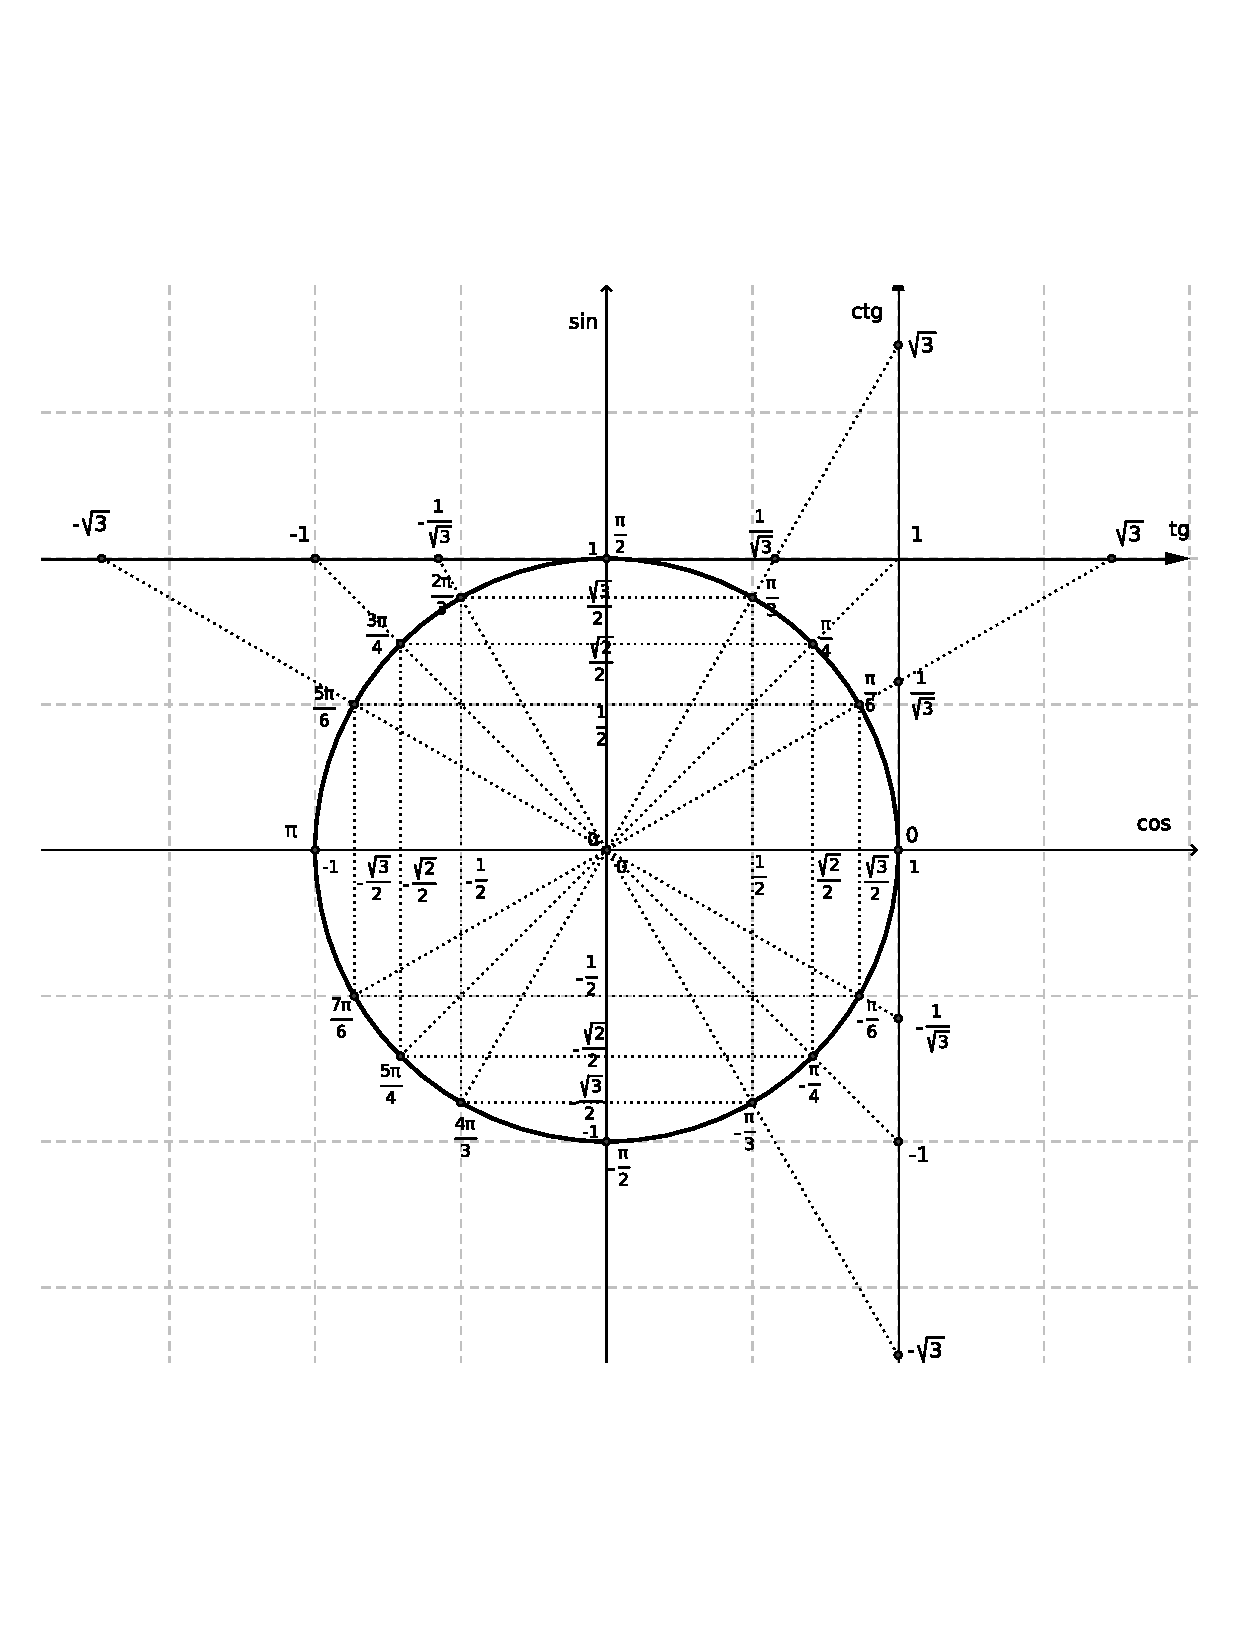
\includegraphics[scale=0.74]{trigokr.pdf}
 % trig.pdf: 1382x1099 pixel, 72dpi, 48.75x38.77 cm, bb=0 0 1382 1099
\end{center}


%
%\newpage\LARGE
%

\section*{������������������ ��������� � ������������ ���������.}
\setcounter{z}{0}

 \textbf{������ ��������� � ������� �����, ������������� ���������� ����������: }

\begin{tabular}{ll}

  % ����� \\: \hline ��� \cline{col1-col2} \cline{col3-col4} ...
 \zad $\sin x=\dfrac13$, \qquad & $[\pi;3\pi]$. \\
  \zad $ 3\cos x=-1$, \qquad & $[\pi;3\pi]$. \\
 \zad $ \tg x=-2$, \qquad & $[-2\pi;\pi].$ \\
 \zad $ \ctg x=5$, \qquad & $[3\pi;4\pi]$. \\
 \zad $ \sin 3x=\sin 3$, \qquad & $[-\pi;0]$. \\
 \zad $2\sin 2x=-\dfrac12$, \qquad & $[2\pi;3\pi]$. \\
 \zad $7\sin 4x+3=0$, \qquad & $[0,5\pi;1,5\pi]$. \\
 \zad $1-4\cos 2x=0$, \qquad & $[4\pi;5\pi]$. \\
 \zad $ 3\cos \dfrac{x}{3}=\dfrac13$, \qquad & $[\pi;7\pi]$. \\
\zad $ \cos 5x=\cos5$, \qquad & $[2,4\pi;3\pi]$. \\
\zad $ 4\cos 4x=-3$, \qquad & $[-\pi;-0,25\pi]$. \\
\zad $ \tg 3x=3$, \qquad & $[-3\pi;-2\pi].$ \\
 \zad $ (\tg^2x-2)(\ctg 2x+2)=0$, \qquad & $[3,5\pi;5\pi].$ \\
 \zad $ (-\tg^24x-2)(4\ctg 4x-12)=0$, \qquad & $[5,5\pi;6\pi].$ \\
 \zad $ (8\sin x+7)(5\cos^3x+1)=0$, \qquad & $[-8\pi;-6,5\pi].$ \\
 \zad $ (27\sin^6 x-1)(27\cos^6x-8)=0$, \qquad & $[2\pi;3\pi].$ \\
 \zad $\dfrac{4\ctg^2x+3\ctg x}{5\cos^2 x-3\cos x}=0,$ & $[2\pi;4\pi].$ \\
 \zad $\dfrac{(41\sin^2x-16)(5\tg x+4)}{\sqrt{41}\cos^2 x-5\cos x}=0,$ & $[2\pi;4\pi].$ \\
 \zad $\dfrac{24\ctg 2x+7}{50\cos^2x-32}=0,$ & $[7\pi;10\pi].$ \\
 \zad $\dfrac{(\cos^44x-\sqrt{3}\cos^34x)(4\ctg^44x-1)}{(\sqrt{3}\sin^44x-\sin^34x)(4\tg^44x+1)}=0,$ & $[1,5\pi;2\pi].$ \\


\end{tabular}


% \newpage \large
% 
\twocolumn[\section*{�����������. ������� � ������������
����������.}] \setcounter{z}{0}

������ �����������:

\zad $2(x+1)<2x+3.$

\zad $x^2\le x.$

\zad $x^2-x+1<0.$

\zad $4x^2+8x+4\ge1.$

\zad $(x+2015)(x-2016)\le0.$

\zad $ -\dfrac{1}{8}\le \dfrac{2x+3}{4}\le-0,25.$

\zad $ \dfrac{4}{7}\le \dfrac{1-3x}{4}\le1,15.$

\zad $ \dfrac{x}{x-3}\le0.$

\zad $ \dfrac{2x+3}{x}\le1.$


\zad $ \dfrac{3x}{x^2-x+2}\le0.$


\zad $ \dfrac{(x-3)^5(x^2-6x+8)}{(x-2)^2(3-x)}\le0.$

\zad $ \left\lbrace
\begin{array}{l}
 2x-1<2,     \\
 3x+1>7.
\end{array}\right.$

\zad $  \left[
\begin{array}{l}
 7x+3>2,     \\
 3>2x-4.
\end{array}\right.$

\zad $  \left\lbrace
\begin{array}{l}
 (x+2)(2-x)<(x+4)(3-x),     \\
 3(3+x)+2(1-2x)\ge12,\\
 (x+2)^2>0.
\end{array}\right.$

\zad $ x\le3-\dfrac{1}{x-1}.$

\zad $ \dfrac{x^2-2x+3}{x^2-1}\ge1.$

\zad $ \dfrac{2}{x-2}> \dfrac{6}{x}-1.$

\zad $   \left\lbrace
\begin{array}{l}
 \dfrac{(3x+1)^2}{2-3x}\le0,     \\
 1\le \dfrac{5x^2-3x+1}{2+x^2}\le3.
\end{array}\right.$

\zad $   \left\lbrace
\begin{array}{l}
 \dfrac{(2x^2-5x+3)(3-x^3)}{x-21}\le0,     \\
 \dfrac{1}{x-8}-\dfrac{1}{x-1}\le1.
\end{array}\right.$

\zad $   \left\lbrace
\begin{array}{l}
 \left[
\begin{array}{l}
 x^2-12x\le0,     \\
 8<x^2,
\end{array}\right.     \\
 \left[
\begin{array}{l}
 3x^2-4x+1\ge0,     \\
 \dfrac{x+2}{x-3}>0.
\end{array}\right.
\end{array}\right.$


\zad $ \left[
\begin{array}{l}
  \left\lbrace
\begin{array}{l}
 x^2+4x-5\ge0,     \\
 6-x>0,
\end{array}\right.     \\
  \left\lbrace
\begin{array}{l}
 x^2-49<0,     \\
 2+x\le0.
\end{array}\right.
\end{array}\right.$

\newpage
\section*{������ ��� ���������������� �������.}
\setcounter{z}{0}

\zad $3(x+1)^2-1\ge 3x^2+6x+2.$


\zad $x^2>4.$

\zad $x^2+x+1>0.$

\zad $9x^2-6x+1<0.$

\zad $(x-2016)(2015-x)>0.$

\zad $ -\dfrac{7}{6}\le \dfrac{4x-5}{9}<-0,24.$

\zad $ \dfrac{4x+3}{2-0,5x}>0.$

\zad $ \dfrac{x+2}{x+1}<2.$

\zad $ \dfrac{x^2-4x+4}{x^2-1}\le0.$

\zad $ \dfrac{x^2-x-6}{3-x}\ge0.$

\zad $ \dfrac{(x^2-7x-8)(x-8)^3}{(x+1)^2(5-x)}\ge0.$

\zad $  \left\lbrace
\begin{array}{l}
 7x+3>2,     \\
 3>2x-4.
\end{array}\right.$

\zad $ \left[
\begin{array}{l}
 2x-1<2,     \\
 3x+1>7.
\end{array}\right.$

\zad $  \left\lbrace
\begin{array}{l}
 x(9x+5)>(1-3x)^2,     \\
 2(5x-3)+3(7-2x)\le32, \\
 (3x-1)^2>0.
\end{array}\right.$

\zad $ \dfrac{x^2-8x+7}{x^2+9x-10}\le1.$

\zad $ \dfrac{7}{(x-2)(x-3)}+\dfrac{9}{x-3}+1<0.$


\zad $  \left\lbrace
\begin{array}{l}
 \dfrac{x^2+10x+25}{4x-4}\ge0,     \\
 (x-2)(x^2-6x+9)\le0, \\
 \dfrac{9-x}{8x}\le1.
\end{array}\right.$

\zad $   \left\lbrace
\begin{array}{l}
 \left[
\begin{array}{l}
 x^2+9x\le0,     \\
 x^2>6,
\end{array}\right.     \\
 \left[
\begin{array}{l}
 2x^2-3x+1\ge0,     \\
 \dfrac{x-1}{x+2}>0.
\end{array}\right.
\end{array}\right.$

\zad $ \left[
\begin{array}{l}
  \left\lbrace
\begin{array}{l}
 x^2+5x-6\ge0,     \\
 7+x>0,
\end{array}\right.     \\
  \left\lbrace
\begin{array}{l}
 x^2-64<0,     \\
 3-x\ge0.
\end{array}\right.
\end{array}\right.$

% 
% \newpage \Large
% \twocolumn[\section*{������ - ������������  �����������.}]
\setcounter{z}{0}

\textbf{������ �����������:}

%\zad $2(x+2)<2x+5.$
%
%
%\zad $ -\dfrac{1}{8}\le \dfrac{2x+3}{4}\le-0,25.$
%
%\zad $ \dfrac{4}{7}\le \dfrac{1-3x}{4}\le1,15.$
%
%\zad $ \dfrac{x}{x-3}\le0.$
%
%\zad $ \dfrac{2x+3}{x}\le1.$
%
%
%\zad $ \dfrac{3x}{x^2-x+2}\le0.$
%
%
%\zad $(x+1)(x-3)(2x+1)(x-7)x>0.$
%
%\zad  $x^4-5x^2+4\geq0.$
%
%
%
% \zad $\dfrac{(x+3)(x-4)x}{(x+1)(x+2)}\le0.$
%
%\zad  $\dfrac{(4+x)^3(x+3)(x-1)^3(x-2)^2}{-3(-5-x)^4(16-4x)^4}>0.$
%
%\zad  $\dfrac{(5-2x)(x+3)}{(2x-7)(6-5x)}\leq0.$


\zad  $\dfrac{(x^2+2x-3)(x^2-16)}{(x^2-1)(x^2-9)}\ge0.$

 \zad $\dfrac{7}{x}>\dfrac{x}{7}.$


\zad  $\dfrac{5}{x}-\dfrac{3}{3-x}<0.$

\zad  $\dfrac{3x+2}{x^2+x-2}<-1.$

\zad  $\dfrac{x^2+4x-1}{x^2+4x+3}\leq\dfrac{1}{x+1}.$

\zad  $\dfrac{x^3-8}{x^3-1}\leq\dfrac{x-2}{x-1}.$

\zad  $\dfrac{1}{2x^2-5x}+\dfrac{4}{25-4x^2}\ge
\dfrac{2}{25+10x}.$


\zad $\dfrac{x^2-4x+3}{x-2}-\dfrac{x-3}{x^2-3x+2}\le0.$

\zad $ x+7+\dfrac{14x-24}{x^2-4x+3}\ge\dfrac{5}{x-1}.$

\zad $\dfrac{x^5-x^2}{x^2}\ge \dfrac{x^3-1}{4x^2}.$

\zad $\dfrac{x^2-5x-6}{x^2-1}\le \dfrac{x-9}{x-1}+\dfrac{2}{x-3}.$


\zad $\dfrac{2-(x-6)^{-1}}{5(x-6)^{-1}-1}\le-0,2.$

\zad  $(x^2-3x-2)(x^2-3x+1)<10.$

\zad  $(x^2+x+1)^2<5x^2+5x-1.$

\zad  $x(x+1)(x+2)(x+3)\leq24.$



\newpage
\section*{������ ��� ���������������� �������.}
\setcounter{z}{0}

%
%
%\zad $x^2>4.$
%
%\zad $x^2+x+1>0.$
%
%\zad $9x^2-6x+1\le0.$
%
%\zad $(x-2011)(2012-x)>0.$
%
%\zad $ -\dfrac{7}{6}\le \dfrac{4x-5}{9}<-0,24.$
%
%\zad $ \dfrac{4x+3}{2-0,5x}>0.$
%
%\zad $ \dfrac{x+2}{x+1}<2.$
%
%\zad $ \dfrac{x^2-4x+4}{x^2-1}\le0.$

\zad $(x^2-3x-4)x>0.$

%\emph{�����:} $ (-1;0)\cup(4;+\infty).$

\zad  $x^4-13x^2+36<0.$

%\emph{�����:} $ (-3;-2)\cup(2;3).$

 \zad
$\dfrac{2-3x}{2x+5}\leq0.$

%\emph{�����:} $ (-\infty;-2,5]\cup[\dfrac{2}{3};+\infty).$

\zad  $\dfrac{9}{x}>\dfrac{x}{4}.$

%\emph{�����:} $ (-\infty;-6)\cup(0;6).$

\zad  $\dfrac{(x+1)(x^2+1)}{(2x-1)(x^2+x+1)}\leq0.$

%\emph{�����:} $ [-1;0,5).$

\zad  $\dfrac{9-x^2}{4x^4-25}\geq0.$

%\emph{�����:} $ [-3;-\sqrt{2,5})\cup(\sqrt{2,5};3].$

\zad  $\dfrac{1}{x}+\dfrac{5}{x+2}<0.$

%\emph{�����:} $ (-\infty;-2)\cup(-\dfrac{1}{3};0).$

\zad  $\dfrac{x^2+2x+3}{x^2-4x+3}>-3.$

%\emph{�����:} $ (-\infty;1)\cup(3;+\infty).$

\zad $x^3+8x^2+\dfrac{50x^2+x-7}{x-7}\le1.$

\zad  $(x^2-x-1)(x^2-x-7)<-5.$

%\emph{�����:} $ (-2;-1)\cup(2;3).$

\zad  $x^2+\dfrac{1}{x^2}\geq1,7\left(x+\dfrac{1}{x} \right) .$

%\emph{�����:} $ (-\infty;0)\cup(0;0,5]\cup[2;+\infty).$

\zad $\dfrac{x^3-3x^2+3x-3}{x^2-3x}\le x+\dfrac{1}{x-2}+\dfrac1x.$

% \newpage \LARGE
% \twocolumn[\section*{����������� � ��������.}] \setcounter{z}{0}

\textbf{\emph{��� ������ ����� ������:}}

\begin{itemize}
    \item $|A|<B \Longleftrightarrow -B<A<B;$
    \item $|A|>B \Longleftrightarrow \left[ \begin{array}{l}
  A>B \\
  A<-B \\
\end{array}  \right.$
 \item $|A|<|B| \Longleftrightarrow A^2<B^2;$
\end{itemize}







\textbf{������ �����������:}

\zad $ |x-2|>2.$

\zad $ |x+1|>-3.$

\hans{\R. }

\zad $ |x-1|\le-4.$

\hans{\O }

\zad $ |x-3|<2.$

\hans{(1;5). }

\zad $ |x^2-1|>0.$

\hans{ (-\infty; -1)\cup(-1;\; 1)\cup(1;+\infty).}

\zad $ ||x-4|-2|<1.$

\zad $ \dfrac{1}{|2-x|}>1.$

\zad $ |x+2|-|x|>0.$

\zad $ |x^2-2x|\ge x.$

\hans{ }

\zad $ |x^2+2x|\le -x.$

\hans{ }

\zad $ |x^2+2x-1|<2x+3.$


%
% \zad $ \dfrac{4x-1}{|x-1|}\ge|x+1|.$

\zad  $|2x^2-9x+15|\geq20.$

 \zad  $1+x+|x^2-x-3|<0.$

  \zad $|x-2x^2|>2x^2-x.$

% \zad  $\left\vert\dfrac{x^2-5x+4}{x^2-4}\right\vert\leq1.$

\zad  $|2x-|x-2||<3.$

\zad  $|2x+1-|3x+1||\leq x+2.$



\newpage
\section*{������ ��� ���������������� �������.}
\setcounter{z}{0}

\zad $ |x+1|>5.$

\hans{ (-\infty; \;-6)\cup(4;+\infty).}


\zad $ |x^2-2x|\le -1.$

\hans{\O }

\zad $ |2x-1|\le 7.$

\hans{  [-3;4].}

\zad $ |x^2-25|\le0.$

\hans{ \pm5.}

\zad $ ||x-5|-3|\ge2.$

\hans{(-\infty;0]\cup[4;6]\cup[10;+\infty).}

\zad $ |x^2+5x|<6.$

\hans{ (-6;-3)\cup(-2;1).}

% \zad $ \dfrac{|x+3|-2}{x+2}\ge2.$
%
% \hans{ [-3;-2).}
%
% \zad $ |x+3|+2|x-1|\le|x|+7.$
%
% \hans{ [-4;3].}

\zad $ \left\vert\dfrac{2x-1}{x+2}\right\vert\le4.$

\hans{(-\infty;-4,5]\cup[-\dfrac{7}{6};+\infty).}


\zad  $|x^2+6x+8|\leq-x^2-6x-8.$

\hans{ [-4;-2].}


\zad $ |x^2-3x+2|\ge|x-1|.$

\hans{ (-\infty;1]\cup[3;+\infty)}


\zad  $||3x+1|+x+1|\geq2.$

\hans{(-\infty;-1]\cup[0;+\infty).}

% \newpage \LARGE
% \twocolumn
[\section*{�������������� �����������.}
\setcounter{z}{0}
{
 \it
$$
 1) \sqrt{f(x)}<g(x) \Longleftrightarrow \left\lbrace \begin{array}{l}
0\leq f(x)<g^2(x)\\
g(x)\geq0
\end{array}
\right.;
 $$
 $$
 2) \sqrt{f(x)}>g(x) \Longleftrightarrow \left[ \begin{array}{l}
{\left\lbrace \begin{array}{l}
f(x)>g^2(x)\\
g(x)\geq0
\end{array}
\right.} \\
{\left\lbrace \begin{array}{l}
f(x)\geq0\\
g(x)<0
\end{array}\right.}
\end{array}\right.
 $$
}
]


\textbf{������ �����������:}


\zad   $\sqrt{x-8}>3.$

\zad   $\sqrt{2-4x}<4.$

\hans{ (-3,5;0,5].}

\zad   $\sqrt{3x-6}<3.$


\zad   $\sqrt{\dfrac{3x-1}{2-x}}>1.$

\hans{  (0,75;2).}


\zad   $\sqrt{2-x}<-x.$

\zad   $\sqrt{x+1}>x-1.$

\hans{  [-1;3).}

\zad   $\sqrt{2x-1}<x.$

\zad   $\sqrt{x^2+3x+2}>3-x.$

\zad   $\sqrt{x+9}>3-x.$


\hans{  (0;+\infty).}


\zad   $x-3\geq\sqrt{9-x^2}.$

\hans{  \{3\}.}


\zad $ \sqrt{3+4x}\ge \sqrt{6x-9}.$


\zad $ \sqrt{22+x}-\sqrt{3-x}<5.$


\zad   $\sqrt{x+2}+\sqrt{3-x}<3.$

\hans{  [-2;-1)\cup(2;3].}


\zad   $\sqrt{x-1}+\sqrt{x+2}\geq3.$


\zad   $\sqrt{2-\sqrt{x+3}}<\sqrt{x+4}.$



\zad   $\sqrt{2x+\sqrt{6x^2+1}}\leq x+1.$


\hans{  \{0\}\cup[2;+\infty).}




\zad   $(9-x^2)\sqrt{x+4}\geq0.$

\hans{  \{-4\}\cup[-3;3].}

\zad   $(x+10)\sqrt{x-4}\leq0.$

\hans{  \{4\}.}

\zad   $(x-12)\sqrt{x-3}\leq0.$

\zad   $(x-3)\sqrt{x^2+x-2}\geq0.$

%
%\zad   $\dfrac{\sqrt{2x^2-5x+2}}{2x^2+6x}\leq0.$
%
%
%\zad
%$\dfrac{\sqrt{4-3x-x^2}}{2x+3}\geq\dfrac{\sqrt{4-3x-x^2}}{x+3}.$
%
%
%\zad
%$\dfrac{\sqrt{6+x-x^2}}{2x+5}\geq\dfrac{\sqrt{6+x-x^2}}{x+4}.$
%
%\hans{ [-2;-1]\cup\{3\}.}
%
%
%\zad   $\sqrt{9-3x}+\sqrt{4-x}>\sqrt{2x+25}.$
%
%
%\zad $$ \sqrt{x^2+4x}+\sqrt{x^2+5x+4}\le\sqrt{2x^2+9x+4}.$$
%
%

% 
% 
% \newpage\Large\onecolumn
% 
\section*{��������������� �������������� � ����������.}
\setcounter{z}{0}

\begin{normalsize}
\textbf{\textit{�������� �������} $(a>0, a\neq1, b>0, c>0)$:}
$$
\begin{array}{lll}
1)\quad  a^{\log_{a}{b}}=b, \quad
&
2)\quad  \log_{a}{a}=1;\quad
&
3)\quad  \log_{a}{1}=0;
\\
4)\quad  \log_{a}{b}+\log_{a}{c}=\log_{a}{bc};\quad
&
5)\quad  \log_{a}{b}-\log_{a}{c}=\log_{a}{\dfrac{b}{c}};\quad
&
6)\quad  \log_{a^m}{b^n}=\dfrac{n}{m}\log_{a}{b}
\\
7)\quad  \log_{a}{b}=\dfrac{1}{\log_{b}{a}}\quad  (b\neq1);\quad
&
8)\quad  \log_{a}{b}=\dfrac{\log_{c}{b}}{\log_{c}{a}} \quad  (c\neq1);
&
9)\quad  b^{\log_{a}{c}}=c^{\log_{a}{b}}.
\end{array}
$$
\end{normalsize}

\textbf{���������: }

\zad $\log_216;$\; $\log_2 \dfrac{1}{8};$ \;$\log_21024;$\;
$\log_21.$
\hans{4;-3;10;0. }

\zad $ \log_{\frac{7}{3}}{\dfrac{3}{7}};$ \;$
\log_{0,2}{\dfrac{1}{25}};$\; $ \log_{2,5}{6 \dfrac{1}{4}};$\; $
\log_{\frac{1}{7}}{343}.$

\hans{-1;2;2;-3. }

\zad $ \lg 1;$\; $ {\lg10000};$ \;$ \lg 0,001$\; $ \lg 100^{100}.$


\zad $ \log_{16}32;$\; $ \log_{625}{125};$ \;$
\log_{7}{7\sqrt{7}};$\; $ \log_{4\sqrt{2}}{\sqrt[5]{16}}.$

\hans{ 1,25;0,75;3/2;0,32.}

\zad $ 8^{\log_{8}{32}};$\; $ 4^{\log_{2}{7}};$\; $
0,5^{\log_{4}{\frac{1}{25}}};$\; $ 5^{\log_{\frac{1}{5}}{4}}.$

\hans{32;49;5;1/4.}

\zad $ \log_{\frac{16}{9}}{\log_{81}{27}};$ \; $
\log^2_{125}{5\sqrt{5}}.$

\hans{ -1/2;1/4.}

\zad $ 100^{\lg 9};$\; $ 7^{\log_{\sqrt[3]{7}}{\lg1000}};$ \;$
\left(\dfrac{1}{9}\right)^{\log_{27}{7\sqrt{7}}};$\; $ \left(\dfrac{1}{2\sqrt{2}}\right)^{\log_{64}{625}}.$

\zad $ {{3}^{2+{{\log }_{3}}15}};
$\;
$ {{4}^{3+{{\log }_{4}}3}};
$\;
 ${{5}^{3+{{\log }_{5}}2}};
$\;
$ {{9}^{\log_{3}4+1}}.
$


\zad $ \lg(49^{\log_{7}{0,8}}+25^{\log_{5}{0,6}});$\; $
6^{\log_{6}{3}+1}-3^{\log_{3}{6}+1}.$

\hans{ 0;0.}

\zad $ \log_{36}{2}+\log_{36}{18};$ \;$ \lg8+\lg125;$\; $ {\log }_{2}3,2+{\log }_{2}5;$\; ${{\log }_{3}}20,25+{{\log }_{3}}4.$

\hans{1;3. }

\zad $ \log_{3}{54}-\log_{3}{6};$ \; $ \log_{2}{72}-\log_{2}{9};$\; $ \log_{\sqrt{2}}{14}-\log_{\sqrt{2}}{7\sqrt{2}};$ \;
$\log_{7}{\log_{2}{16}}-\log_{7}{28}.$

\hans{ 2;3;1;-1.}

\zad $\log_5{0,25}-2\log_5\dfrac23+\log_5\dfrac{16}{9};$\; $\log_38-2\log_32+\log_3\dfrac92.$

\zad $ \dfrac{\log_{2}{27}}{\log_{2}{9}};$ \; $
\dfrac{\log_{7}{9}}{\log_{\sqrt{7}}{9}};$\; $ \dfrac{\log_{5}{2}+\log_{5}{3}}{\log_{5}{36}};$ \; $
\dfrac{\log_{5}{49}}{\log_{5}{21}-\log_{25}{9}}.$

\hans{ 3/2;1/2;1/2;2.}

\zad $ \dfrac{{{\log }_{8}}20}{{{\log }_{8}}5}+{{\log }_{5}}0,05;$\; $ \dfrac{{{\log }_{2}}600}{{{\log }_{2}}12}+{{\log }_{12}}0,02.
$

\zad $ \log_{5}{3}\cdot\log_{3}{5};$ \; $ \log_5128\cdot\log_2125;$\; $49^{\frac{1}{2\log_97}};$\;
$
27^{\frac{1}{\log_{2}{3}}}+9^{\frac{1}{\log_{5}{3}}}.$

\hans{1;33. }

\zad $ \log_{2}{(\log_{\sqrt{2}}{9}\cdot\log_{\sqrt{3}}{2})};$ \; $
\dfrac{\log_{3}{37}}{\log_{21}{37}}-\log_{3}{7};$\; $
\dfrac{\log_{12}{30}}{\log_{3}{30}}+\log_{12}{4};$\; $ \log_{3}{\sqrt{\log_{5}{4}}}+\log_{9}{\log_{64}{5}}.$ \;

\zad
$\dfrac{\log_2^214+\log_214\cdot\log_27-2\log_2^27}{\log_214+2\log_27};$\; $
\dfrac{\log_{4}{(\sqrt{3}-\sqrt{5})^2}+\log_{2}{(\sqrt{3}+\sqrt{5})}}{27^{\frac{1}{3}-\frac{1}{2}\log_{3}{4}}+2^{\frac{1}{\log_{8}{0,5}}}}.$





\zad $ 2^{\frac{\log_{2}{5}}{\log_{5}{2}}}-5^{\log_{2}{5}};$\; $3^{2+\frac{\log_34}{\log_43}}-9\cdot4^{\frac{1}{\log_43}}+4^{1+\log_425}.$



\textbf{������� �������� ���������:}

\zad $ \log_{6}{(18a)},$ \; ���� \;  $ \log_{6}{3a}=0,3.$

\hans{ 1,3.}

\zad $ 2\lg a+\lg b,$ \; ���� \; $ \lg(0,001a^2b)=2,5.$

\hans{ 5,5.}

\zad $ \log^2_{\sqrt[3]{a}}{b}+\log_{\sqrt[3]{b}}{a},$ \; ���� \;
$ \log_{b}{a}=3.$

\hans{ 10.}


\zad $ \log_{\frac{\sqrt{b}}{a^2}}\dfrac{\sqrt{a}}{\sqrt[4]{b}}+\dfrac14\log_{\frac{\sqrt{b}}{a^2}}{b\sqrt{a}},$ \; ���� \;
$ \log_{a}{b}=14.$


\zad $ \log_{a}{b},$ \; ���� \; $ \log^2_{a^2b}{ab^2}=4.$

\hans{ -1,25.}

\zad $
\log_{ab}{\dfrac{\sqrt{b}}{a}}+\log_{\sqrt{ab}}{b}+\log_{a}{\sqrt[3]{b}},$
 ���� $ \log_{b\sqrt{a}}{\dfrac{b}{a}}=\dfrac{2}{5}.$

\hans{ 2.}

\zad  $
(\log_{4}{6}+\log_{6}{4}+2)(\log_{4}{6}-\log_{24}{6})\log_{6}{4}-\log_{4}{6}.$\; 

\hans{1. }


% 
% \newpage\LARGE
% \section*{�������������  �����������.}
\setcounter{z}{0}


\zad $ 8^{5-\frac x3}>4.$

\zad $\dfrac18\cdot\left(\dfrac12\right)^{x(2-x)}> 8\cdot
\left(\dfrac12\right)^{3x}.$

\zad $\dfrac{(\sqrt5)^{x-10}}{4^{x-10}}> \dfrac{5\sqrt5}{64}.$

\zad $\dfrac{0,2^{x+0,5}}{\sqrt5}> \dfrac{0,04^x}{25}.$

\zad $ 4^x-4^{x-1}<3.$

\zad $\dfrac{7^x-35}{7^{x-1}+1}\le -14.$

\zad $2^{x+2}-2^{x+3}-2^{x+4}>5^{x+1}-5^{x+2}.$

\zad $9\cdot3^{2x+2}+3\cdot3^{2x+1}-9^x\le89.$

\zad $ 3^{1+x}\cdot2^{1-x}+3^{x}\cdot2^{-x}<10,5.$

\zad $ 3^{x+2}\cdot2^{1-2x}\le20.$

\zad $ 3^{2x-1}<11^{3-x}.$

\zad $9^{x-1}-36\cdot 3^{x-3}+3<0.$

\zad $2^{2x+1}-21\cdot\left(\dfrac12\right)^{2x+3}+2\ge 0.$

\zad $2\cdot 3^{2x^2}+4\le 3^{x^2+2}.$

\zad $0,25^{\sqrt x} < 2^{3-\sqrt x}+25^{\log_3^{-1}5}.$

\zad $3^{\sqrt x}-3^{1-\sqrt x}\le \dfrac{26}3.$

\zad $4^{\sqrt x} -2^{\sqrt x+1}< 2^{\sqrt x+4} -32.$

\zad $15\cdot 2^{2-2x}+19\cdot 2^{-x}>2.$

\zad $4\cdot 3^{x+2}-2\cdot 5^{x+2} \le 5^{x+3}-3^{x+3}.$


\zad $5\cdot 9^x-18\cdot 15^x+9\cdot 25^x>0.$

\zad $ 16^x-2\cdot12^x\le3^{2x+1}.$

\zad $4^{x^2-x}-10\cdot 2^{x^2}+2^{2x+4}\ge 0.$


\zad $ 3^{x-1}\ge\dfrac{2-3^x}{3^x-4}.$


\zad $ (\sqrt{3}-\sqrt{2})^{3-x}\le
(\sqrt{3}+\sqrt{2})^{\sqrt{x+3}}.$

%% \emph{�����: } $ [-3;6].$


\zad $ \big| |3^x+4x-9|-8\big|\le3^x-4x-1.$

% \onecolumn
% \newpage\Large
% 
\section*{��������������� �����������.}
\setcounter{z}{0}

\begin{normalsize} \textbf{\textit{�������� ��������������� �������}}\quad
$y=\log_ax$ \; ${(a>0,\; a\neq1)}:$
\begin{enumerate}
\item ������� ����������� ������� --- ��������� ���� �������������
�������������� ����� ($x>0$). \item ������� �������� ������� ---
��������� ���� �������������� �����. \item  ��� $a>1$ �������
����������:\quad $0<x_1<x_2\Longleftrightarrow
\log_a{x_1}<\log_a{x_2}$. \item  ��� $0<a<1$ ������� �������:
\quad $0<x_1<x_2\Longleftrightarrow {\log_a{x_1}>\log_a{x_2}}$.
% \item $\log_a{x_1}=\log_a{x_2}\Longleftrightarrow x_1=x_2>0.$
% \item $\log_a{a^x}=x$ ��� ���� $x\in\R$, \quad $a^{\log_ax}=x$ ���
% ���� $x>0.$
\end{enumerate}
\end{normalsize}

\zad $ \log_{0,7}(2x-3)>\log_{0,7}(6-x).$

\hans{ (1,5;3).}

\zad $ 10^{\lg\log_2x}+\log_2x\le4.$

% \zad $ \log_7(x-1)>\log_7(2x-5).$
% 
% \hans{ (2,5;4).}


% 
% \zad $\log_2(x^2+3x)\le 2.$
% 
% \zad $\log_{1/3}\left(\dfrac{2-3x}{x} \right)\ge -1.$
% 
% \zad $\log_3(x^2-x)\le \log_3(3x+2).$

\zad $\log_7x\cdot\log_37<5.$


\zad $\log_5x\cdot\log_{0,3}5<\log_{0,3}4.$


\zad $\log_{1/\sqrt 5}(x^2-0,8x)\ge 2.$

\hans{ [-0,2;0)\cup(0,8;1].}

% \zad $ \log_{\pi-3}(x^2+x+31)\le\log_{\pi-3}(10x+11).$
% 
% \hans{ (-1,1;4]\cup[5;+\infty).}
% 
% 
% \zad  $\log_{0,1}(x^2+x-2)>\log_{0,1}(x+3). $
% 
% \hans{(-\sqrt{5};-2)\cup(1;\sqrt{5}) }

\zad $ \log_4(x-3)+\log_2(x-3)< \dfrac{3}{2}.$

% \zad $ \log_{\frac{1}{3}}(x-2)+\log_{\frac{1}{3}}(x+24)>-3.$
% 
% \zad $ \log_2(x-1)\le1+\log_{0,5}x.$

\zad $\log_5 x+\log_{25}x<\log_{1/5}\sqrt{125}.$

\zad $ \log_{\log_32}(2x-3)>0.$

% 
% \zad $ \log_{\frac{1}{3}}\log_2(x^2-3)>0.$
% 
% \hans{ (-\sqrt{5};-2)\cup(2;\sqrt{5}).}


% \zad $\log_2(\log_{1/3}(\log_5x))>0.$
% 
% 
% \zad   $ \left(\dfrac12 \right)^{\log_5(x^2-1)}>1.$
% 
% \hans{(-\sqrt{2};-1)\cup(1;\sqrt{2}) }
% 
% \zad $ \log_2(x-2)+\log_4(x-3)^2\le1.$
% 
% \hans{ (3;4].}
% 
% \zad $ \log_2(x^2-3x)\le5+\log_{0,5}(x+4).$
% 
% \hans{ (-4;0)\cup(3;4].}
% 
% \zad $ \log_3(3-x)+\log_3(5-x)>\log_3(x+7).$
% 
% \hans{ (-7;1).}
% 
% \zad $ \log_{0,1}(x-1)+\log_{0,1}(x-2)\ge\log_{0,1}(x+2).$
% 
% \hans{ (2;4].}
% 
% \zad $ \log_{0,3}\dfrac{x+10}{x-2}\le\log_{0,3}(x+3).$
% 
% \zad $
% \log_{\sqrt{3}}\sqrt{x-1}+\log_{\frac{1}{3}}3\le\log_{\frac{1}{3}}(x+4)+\log_94.$
% 
% \zad $ \log_2(x+3)+\log_2(x^2-4x+1)\ge\log_2(11-x).$
% 


% \zad   $ \log_3((x+2)(x+4))+\log_{\frac{1}{3}}(x+2)< \dfrac12\log_{\sqrt{3}}7.$
% 
% \hans{(-2;3) }
% 
% 
% \zad $\log_3(x^2+7x+10)+\log_{\frac13}\dfrac{x+5}{9}+1\ge\log_3(3x^2+16x+20).$
% 
% 
% \zad   $\log_5(x+2)+\log_5(1-x)\le\log_5((1-x)(x^2-8x-8)). $
% 
% \hans{ (-2;-1]}

\zad   $\log_2\dfrac{3x-2}{x-1}+3\log_8\dfrac{(x-1)^3}{3x-2}<1. $

\hans{ (1-\sqrt{2};-2/3)\cup(1;1+\sqrt{2})}

\zad $\log^2_2(5-x)-6\log_2(5-x)+9\le 0.$

\zad $\dfrac1{\log_2 x-4}>\dfrac1{\log_2x}.$

\hans{ (0;1)\cup(16;+\infty).}

\zad $\dfrac4{\lg 10x}-\dfrac5{\lg100x}\ge 0.$


\zad   $\dfrac{\log_2x-5}{1-2\log_2x}\ge2\log_2x.$

\hans{ (0;0,5]\cup(\sqrt{2};2\sqrt[4]{2}]}


\zad $ \log_{\frac{1}{2}}x\cdot\log_2x+\log_{\frac{1}{2}}x+2\le0.$

\hans{ (0;0,25]\cup[2;+\infty).}

\zad $ \log^2_{0,5}x-3>2|\log_{0,5}x|.$

\hans{ (0;1/8)\cup(8;+\infty).}


\zad $\log_9x^2+\log^2_3(-x)<2.$

\zad $
\log_{x-4}(2x-9)\cdot\log_{2x-9}\pi\le\log_{x-4}(x-3,8)\cdot\log_{x-3,8}3.$

\hans{ (4,5;4,8)\cup(4,8;5).}

% \zad $
% \log_3x<(\log_3x\cdot\log_372-\log_3576)\cdot\log_{\frac{x}{3}}3.$
% 
% \hans{ (0;3)\cup(9;24).}


\zad $ \log_7x\cdot\log_3x-\log_73\cdot\log_3x\le12\log_73.$

\zad $ \log_3x\cdot\log_{0,3}x+\log_3{0,3}\cdot\log_{0,3}x>6\log_3{0,3}.$



% 
% \zad $ \log_{x^2+2}(3x+12)>1.$

\zad $ \log_{1-x^2}(5x+5)<1.$

% 
% \zad $(4x-1)\log_2x\ge 0.$
% 
% \hans{ (0;0,25]\cup[1;+\infty).}
% 
% \zad $ x\log_3x-\dfrac{3}{\log_x3}\le0.$
% 
% 
% \zad $ x\log_2 \left(\dfrac{x}{3}+2
% \right)\le10\log_{\frac{1}{4}}\left( \dfrac{x}{3}+2\right).$
% 
% \hans{ [-5;-3].}

\zad $ \log_{x^2}5>\log_{x^2}7.$

\zad $ \dfrac{\log_{27}x}{\log_3(1+2x)}\le
\dfrac{\log_3\sqrt[3]{2x+1}}{\log_3x}.$

\zad $\log_x3<1.$

 \zad $\log_{0,5}{(2^x-1)}>x-1.$

 \zad
$\log_{9x}{3}\ge\log^2_{x}{3}.$

% \zad $\sqrt{1-\log_{1/2}x} <2.$

\zad $\sqrt{\log_3(9x+27)}\ge\log_3(x+3).$


\zad $\dfrac{\sqrt {2x+1}}{2+\log_{1/2}(x+1)}\ge 0.$



% 
% 
% \zad $\log_{x}\log_2(4^x-12)\le 1.$
% 
% 
% \zad   $ \log_x(\log_9(3^x-9))<1.$
% 
% \hans{(\log_310;+\infty) }
% 
% \zad   $ \log_{\frac{x}{3}}(\log_x\sqrt{3-x})\ge0.$
% 
% \hans{ \left[\frac{\sqrt{13}-1}{2};2 \right)}

% 
% \zad $ \log_8(2-x)+\log_8(x^3-x+2)\ge\log_82x^3.$
% 
% \hans{ (0;1].}
% 
% 
% \zad $ \log_x(x^3-8x^2+19x-10)>\log_x(5-x)+\log_x(x-2). $
% 
% \hans{ }


\zad   $x^{\lg x}<1000x^2.$

\zad  $ x\cdot2^{\log_{x}{5}}\ge10.$

\zad   $3^{\log^2_{3}{x}}+x^{\log_{3}{x}}\le162.$





% \newpage
% \twocolumn
[\section*{����� �������������� 1.}
\setcounter{z}{0}
{
 \it ���� ������� $f(x)$ ����������, �� ��������� $f(A)-f(B)$ ����� ����� �� ����, ��� � ��������� $A-B$. � ���������, ��� $A\ge0$ � $B\ge0$ ����� ��������� $A-B$ � $A^2-B^2$ ���������, �.�. $sign(|A|-|B|)=sign(A^2-B^2)$, � $sign(\sqrt{A}-\sqrt{B})=sign(A-B)$.
}

\bigskip
]

\textbf{������ �����������:}


\medskip \zad $(|x-1|-1)(|x-3|-2)<0.$


\medskip \zad $\dfrac{|x+3|+3}{|x-2|-2}>0.$

\medskip \zad $ \dfrac{1}{|x+1|-1}\ge\dfrac{2}{|x+1|-2}.$

\medskip \zad $ \dfrac{|x-1|-|2x+1|}{|x-2|-|2x+2|}\ge0.$

\medskip \zad $ \dfrac{4|2-x|}{4-|x|}-|x-2|\le0.$

\medskip \zad $ \dfrac{|x-4|-2-x^2}{|2+x|-|x-6|}>0.$

\medskip \zad $ \dfrac{|4x-3|-|3x-4|}{|x^2-x-18|-|x^2+x|}\le0.$

\medskip \zad $ \dfrac{||x^2+x|-3|-3}{||3x+4|-2|-1}\ge0.$

\medskip \zad $ |x^2-5|x|+4|\le |2x^2-3|x|+1|.$

\medskip \zad $ \dfrac{|2x^2-5x|-x^2}{|3x^2-5x|-x^2}\le0.$

\medskip \zad $ \dfrac{|2x^2-x-3|-x^2-2x-1}{|3x^2+x-2|-x^2-2x-1}\le0.$

\medskip \zad $ \dfrac{(x-2)^2-3|x-2|-10}{(|x-4|-5)(|3-x^2|-6)}\ge0.$

\medskip \zad $ \dfrac{(|x^2-4|-5)(|x+5|-8)}{(|x-3|-|x-1|)|x|}\ge0.$

 \medskip \zad $ \dfrac{|x-3|-2}{|x|-1}\le2.$



\medskip \zad   $\dfrac{\sqrt{2x^2-5x+2}}{2x^2+6x}\leq0.$



\medskip \zad
$\dfrac{\sqrt{6+x-x^2}}{2x+5}\geq\dfrac{\sqrt{6+x-x^2}}{x+4}.$

\hans{ [-2;-1]\cup\{3\}.}


\medskip \zad $ \dfrac{\sqrt{x^2-9}-\sqrt{2(5x+1)}}{\sqrt{x+3}-2}\le0.$

\medskip \zad $ \dfrac{\sqrt{2x+3}+x-6}{x-5}\ge3.$

\medskip \zad $ \dfrac{\sqrt{8-x}-|2x-1|}{\sqrt{x+7}-|2x-1|}\le1.$

\medskip \zad $ \dfrac{|x+5|-\sqrt{2x+18}}{|x-4|-\sqrt{12-3x}}\ge0.$

\medskip \zad $ (\sqrt{3x+5}-\sqrt{x+3})(|x-4|-x^2-2)<0.$

\medskip \zad $ \dfrac{\sqrt{3x^2-5x+3}-\sqrt{x^2+x+1}}{|2x^2-x-1|-|12x^2+7x+1|}\ge0.$

\medskip \zad $$ |\sqrt{x^2+x+1}-2x-1|-|\sqrt{x^2+x+1}+2x+2|>0.$$

\medskip \zad $$ \dfrac{\sqrt{x+\sqrt{3x-2}}-\sqrt{x+\sqrt{2x-3}}}{\sqrt{x-2\sqrt{x-1}}-\sqrt{x+3-4\sqrt{x-1}}}\le0.$$

\medskip \zad $ \dfrac{\sqrt{2x^2+x+1}-\sqrt{x^2+x+1}}{\sqrt[3]{3x^2+4x-2}+\sqrt[3]{3x^2+x-4}}\ge0.$

\medskip \zad $ \dfrac{|x+1|-\sqrt{5-2x-2x^2}}{\sqrt[3]{x^3+2x^2-5x+2}-x}\le0.$

\medskip \zad $$ \dfrac{(\sqrt{1+2x^2}-1-x^2)\cdot(|2x+3|-|3x+2|)}{(x^2-5x+4)\cdot(\sqrt{x+5}+1-x)\cdot(x^{99}-1)}\le0.$$

\medskip \zad $$ \dfrac{((2x-1)^5-(x+1)^5)\cdot(\sqrt[3]{x^2-6}+\sqrt[3]{x})}{\sqrt{x^2+x+1}-\sqrt{x^2+2}}\le0.$$

\medskip \zad $ \dfrac{\sqrt[3]{(x-1)^2}-\sqrt[3]{x-1}-2}{|x+3|-\sqrt{x^2-2x-3}}\le0.$

\medskip \zad $$ \dfrac{(\sqrt{7-x}-x-5)\cdot(\sqrt{11-4x}-x-2,5)}{\sqrt{5+3x-2x^2}\cdot(|4x-3|-|6x+1|)}\le0.$$



% \newpage
% \onecolumn
\section*{����� �������������� 2.}
\setcounter{z}{0}

%\begin{normalsize}
��� ���� ���������� ��������� ���������� $a,$ $b$ � $c$
\begin{itemize}
 \item $\log_ab$ ����� ����� �� ����, ��� � ��������� $(a-1)(b-1)$;
\item $\log_ab-\log_ac$ ����� ����� �� ����, ��� � ��������� $(a-1)(b-c)$;
\item $a^b-a^c$ ����� ����� �� ����, ��� � ��������� $(a-1)(b-c)$.
\end{itemize}
%\end{normalsize}


  
 \zad $ \dfrac{\log_2(2x)\cdot\log_{0,5x}x^2}{\log_{0,125x}8}\le0.$

\zad   $\log_{2-x}(x+2)\cdot\log_{x+3}(3-x)\le0. $

\zad $\log_{\sqrt{2x^2-7x+6}}\left(\dfrac{x}{3}\right)>0.$
\hans{(1;1,5)\cup(2;2,5)\cup(3;+\infty) }


\zad $\log_{\log_2(x/2)}(x^2-10x+22)>0.$


\zad   $ \log_{\frac{3x-1}{x+2}}(2x^2+x-1)\ge\log_{\frac{3x-1}{x+2}}(11x-6-3x^2).$

\zad $\log_{\frac{2x-1}{x}}5<\log_{\frac{2x-1}{x}}x.$
\hans{ (0,5;1)\cup(5;+\infty)}  

\zad   $\log_{6x^2-5x+1}2>\log_{\sqrt{6x^2-5x+1}}2. $
\hans{ (0;1/3)\cup(1/2;5/6)} 

\zad $\log_{x^2}(9-8x)\ge1.$ 

\zad   $ \log_{2x+3}x^2<1.$
\hans{ (-1,5;-1)\cup(-1;0)\cup(0;3)} 

\zad   $ \dfrac{2\log_{2^{x-1}}|x|}{\log_{2^{x-1}}(x+7)}\le \dfrac{\log_3(x+12)}{\log_3(x+7)}.$

\zad   $\dfrac{\log_2(2x^2-13x+20)-1}{\log_3(x+7)}\le0. $

\zad $ \dfrac{2\log_3(x^2-4x)}{\log_3x^2}\le1.$

\zad $ \log_{\frac{1}{36}}(22-3x)\cdot\log_{8-x}\dfrac16\ge1.$

\zad   $ \log_{|x+2|}(4+7x-2x^2)\le2.$

\zad $\dfrac{9}{\log_{1,9}x\log_{2,1}(x-10)^2}\ge \dfrac{(x-1)^{\log_3(x-1)}}{9\log_{1,9}x\log_{2,1}(x-10)^2}.$

\zad   $ \dfrac{\log_2(3\cdot2^{x-1}-1)}{x}\ge1.$

\zad $\dfrac{12^x-4^{x+1}-3^{x+1}+12}{x^2-2x+1}<0.$

\zad $ |x|^{x^2-x-2}>1.$


\zad $ |x+1|^{x^2+5x}\ge1.$
% \emph{�����: } $ (-\infty;-5]\cup[-2;-1)\cup(-1;+\infty).$
 
\zad $6^x\ge 3\sqrt 3\cdot 2^x+32\cdot 2^2\cdot 3^x-64\sqrt{108}.$

\zad $ x^2\cdot2^{x+2}-12x^2\cdot3^x+3^{x+1}>2^x.$

\zad $\sqrt{6-x}\cdot(2\cdot 9^{2x}-53\cdot 3^{2x}-27)\ge 0.$

\zad $\dfrac{x+1-\log_3 9x}{1-\log_3x}\ge1.$


\zad $ \dfrac{(7x-x^2+98)\sqrt{x+6}}{\log_2{|x-12|}-4}\ge0.$

\zad $
\log_{0,5x-2}{\left(\log_4{\left(\dfrac{12}{\sqrt{3x-12}}\right)}\right)}\le0.$



\zad $\log_{3x-5}{2}\le\log_{x-1}{\sqrt{2}}.$

\zad $ \lg^2\dfrac{(x-3)^2\cdot(x-2)}{18}>\lg^2\dfrac{(x-2)}{2}. $

%\zad $\dfrac{\log_{2^{x+4}}4}{\log_{2^{x+4}}(-8x)}\le\dfrac{1}{\log_2\log_{\frac12}2^x}.$

% \newpage
% 

\section*{������� ���� �3.}
\setcounter{z}{0}


\medskip \zad (���2010)  $ \log_5((7^{-x^2}-6)(7^{-x^2+16}-1))+\log_5\dfrac{(7^{-x^2}-6)}{7^{-x^2+16}-1}>\log_5(7^{2-x^2}-5)^2.$

\hans{ (-\infty;-4)\cup(4;+\infty)}

% \medskip \zad (���2010)  $ \log_2((5^{-x^2}-3)(5^{-x^2+9}-1))+\log_2\dfrac{(5^{-x^2}-3)}{5^{-x^2+9}-1}>\log_2(5^{4-x^2}-2)^2.$


\medskip \zad (���2011) $ 11\cdot\lg(x^2+11x+30)\le 12+\lg\dfrac{(x+6)^{11}}{x+5}.$


 \medskip \zad (���2011) $ 3\log_{11}(x^2+8x-9)\le 4+\log_{11}\dfrac{(x-1)^{3}}{x+9}.$


\medskip \zad (���2011) $\log_4(x+5)^4\cdot\log_{16}(x+4)^2+\log_2\dfrac{(x+4)^3}{x+5}-3>0.$



 \medskip \zad (���2011)  $\log_8(x-3)^2\cdot\log_{16}(x-7)^6+\log_2\dfrac{(x-3)^5}{x-7}-5>0.$




%\medskip \zad $2\log_{0,5x+0,5}x^2+\log_{|x|}(0,5x+0,5)\le4.$


\medskip \zad (���2011)  $2\log_{1-0,5x}(x-1)^2+\log_{|x-1|}(1-0,5x)\le4.$


\medskip \zad  (���2011)   $ \log_{x+1}(19+18x-x^2)-\dfrac1{16}\log^2_{x+1}(x-19)^2\ge2.$

\hans{ 3}


\medskip \zad (���2011)   $ \dfrac12\log_{x+4}(x^2+2x+1)+\log^2_{-x-1}(-x^2-5x-4)\le-1.$





\medskip \zad (��� 2012) $\left\{ \begin{array}{l}
                \dfrac{160-4^x}{32-2^x}\ge5, \\
                \log_{0,25x^2}\left(\dfrac{6-x}{4} \right)\le1.
              \end{array}
 \right.$

\medskip \zad (��� 2012) $\left\{ \begin{array}{l}
                11^{x+1}+3\cdot11^{-x}\le34, \\
                \log_{2x}0,25\le\log_232x-1.
              \end{array}
 \right.$


\medskip \zad (��� 2013) $\left\{ \begin{array}{l}
                x+7+\dfrac{14x-24}{x^2-4x+3}\ge\dfrac{5}{x-1}, \\
                \log_{4-x}\left(28-3x-x^2 \right)\le1.
              \end{array}
 \right.$

\medskip \zad (��� 2013) $\left\{ \begin{array}{l}
                x^3+8x^2+\dfrac{50x^2+x-7}{x-7}\le1, \\
                \log_{5-x}\dfrac{x+4}{(x-5)^{10}}\ge-10.
              \end{array}
 \right.$
 

 \medskip \zad (��� 2014) $\left\{ \begin{array}{l}
                \log_{11-x}(x+7)\cdot\log_{x+5}(9-x)\le0, \\
                 64^{x^2-3x+20}-0,125^{2x^2-6x-200}\le0.
              \end{array}
 \right.$

\medskip \zad (��� 2014) $\left\{ \begin{array}{l}
                32\cdot9^{x}\le60\cdot3^x-7, \\
                 \log_{7-x}(x+2)\le\log_{7-x}(3-x).
              \end{array}
 \right.$

 
 \medskip \zad (��� 2015) $\dfrac{105}{\left(2^{4-x^2}-1 \right)^2}-\dfrac{22}{2^{4-x^2}-1}+1\ge0.$
 
 
 
 \medskip \zad (��� 2015) $\lg^4x-4\lg^3x+5\lg^2x-2\lg x\ge0.$
 
 
 \medskip \zad (��� 2015) $\left( \log^2_2x-2\log_2x \right)^2<11\log^2_2x-22\log_2x-24.$
 
 
 \medskip \zad (��� 2015) $\dfrac{31-5\cdot2^x}{4^x-24\cdot2^x+128}\ge0,25.$
 
% % \newpage
% % 

\section*{������ ��� ���������������� �������.}
\setcounter{z}{0}


\medskip \zad (���2010)  $ \log_2((5^{-x^2}-3)(5^{-x^2+9}-1))+\log_2\dfrac{(5^{-x^2}-3)}{5^{-x^2+9}-1}>\log_2(5^{4-x^2}-2)^2.$



\medskip \zad (���2011) $ 3\log_{11}(x^2+8x-9)\le 4+\log_{11}\dfrac{(x-1)^{3}}{x+9}.$




\medskip \zad (���2011)  $\log_8(x-3)^2\cdot\log_{16}(x-7)^6+\log_2\dfrac{(x-3)^5}{x-7}-5>0.$




\medskip \zad (���2011) $2\log_{0,5x+0,5}x^2+\log_{|x|}(0,5x+0,5)\le4.$



\medskip \zad  (���2011)   $ \log_{x+1}(19+18x-x^2)-\dfrac1{16}\log^2_{x+1}(x-19)^2\ge2.$

\hans{ 3}





\medskip \zad (��� 2012) $\left\{ \begin{array}{l}
                11^{x+1}+3\cdot11^{-x}\le34, \\
                \log_{2x}0,25\le\log_232x-1.
              \end{array}
 \right.$
\\

\medskip \zad (��� 2013) $\left\{ \begin{array}{l}
                x^3+8x^2+\dfrac{50x^2+x-7}{x-7}\le1, \\
                \log_{5-x}\dfrac{x+4}{(x-5)^{10}}\ge-10.
              \end{array}
 \right.$
 \\

\medskip \zad (��� 2014) $\left\{ \begin{array}{l}
                32\cdot9^{x}\le60\cdot3^x-7, \\
                 \log_{7-x}(x+2)\le\log_{7-x}(3-x).
              \end{array}
 \right.$

 
 \medskip \zad (��� 2015) $\dfrac{31-5\cdot2^x}{4^x-24\cdot2^x+128}\ge0,25.$
 
 
% 
% \newpage
% 

\section*{������������������ ���������.}
\setcounter{z}{0}

 \textbf{������ ���������: }

\begin{tabular}{lll}

  % ����� \\: \hline ��� \cline{col1-col2} \cline{col3-col4} ...
 \zad $ \sin x=0.$ & \zad $\cos x=0. $
 &\zad $ \tg x=0.$
 \\
  \zad $\ctg x=0. $ & \zad $ \sin x=1.$ & \zad $ \cos x=-1$. \\
  \zad $\sin x=-\dfrac{1}{2}.$ & \zad $\ctg x=\sqrt{3}.$
 & \zad $\sin3x=\dfrac{\sqrt{3}}{2}.$\\
  \zad $\cos 2x=\dfrac{\sqrt{3}}{2}.$ & \zad $\tg \dfrac{2x}{5}=1.$ & \zad $ 2\cos (\dfrac{x}{2}-\dfrac{\pi}{6})=\sqrt{3}.$ \\
  \zad $ 2\sin(3x-\dfrac{\pi}{4})=-\sqrt{2}.$ & \zad $ \sqrt{3}\tg(\dfrac{x}{3}+\dfrac{\pi}{3})=3.$ & \zad $ \ctg \dfrac{\pi x-\pi}{4}=1.$ \\

\end{tabular}


\zad $\sqrt{3}+2\cos \dfrac{\pi x}{9}=0 $\; �� ���������� \;
$8<x<30.$


\hans{ 10,5.}

\zad $1-\sqrt{2}\sin \dfrac{\pi x}{4}=0$\; �� ���������� \;
$1<x<10.$

\hans{3.}


\textbf{������ �������:}

\begin{tabular}{ll}
  \zad
 $\left\{ \begin{array}{ll}
  x=\dfrac{\pi}{3}+\dfrac{2\pi n}{3}, & \; n\in\Z; \\
  x=\pi k, & \; k\in\Z. \\
\end{array}\right.$ & \zad
 $\left\{ \begin{array}{ll}
  x=\dfrac{\pi}{4}+\dfrac{\pi n}{2}, & \; n\in\Z; \\
  x=(-1)^k \dfrac{\pi}{4}+\pi k, & \; k\in\Z. \\
\end{array}\right.$
 \\
  \zad
 $\left\{ \begin{array}{ll}
  x=\pm\dfrac{\pi}{3}+2\pi n, & \; n\in\Z; \\
  x\neq (-1)^k \dfrac{\pi}{3}+\pi k, & \; k\in\Z. \\
\end{array}\right.$
 & \zad
 $\left\{ \begin{array}{l}
  \sin2x=0 \\
  \cos \dfrac{x}{2}\neq0. \\
\end{array}\right.$
 \\
  \end{tabular}




\textbf{������ ���������:}

\begin{tabular}{lll}

  \zad $\dfrac{\cos x}{1-\sin x}=0.$&\hspace{40mm} & \zad $\dfrac{\sin(x-\frac{\pi}{4})}{\cos x-\frac{\sqrt{2}}{2}}=0.$ \\
  \zad $ \dfrac{\cos x-0,5}{\cos(x+\frac{\pi}{6})}=0.$& \hfill &\zad $ \dfrac{\cos x+\frac{\sqrt{3}}{2}}{\sin x-0,5}=0.$ \\
  \zad $ \dfrac{2\cos^2x-1}{\tg x+1}=0.$& & \zad $ \cos x (\tg^2x-\dfrac{1}{3})=0.$ \\
  \zad $ \dfrac{4\sin^2x-3}{\tg x-\sqrt{3}}=0.$& & \zad $ \dfrac{4\cos^3x-\cos x}{\tg x-\sqrt{3}}=0.$ \\
 \end{tabular}


\zad ������� ��� ����� ��������� $ (2\sin x+1)(2\sin x-\sqrt{3})=0,$ ��������������� ����������� $ \cos x>0.$

\zad ������� ��� ����� ��������� $ (\sqrt{2}\sin x+1)(2\sin x-3)=0,$ ��������������� ����������� $ \tg x<0.$


\zad ������� ��� ����� ��������� $ (\sqrt2\cos x-1)(2\cos x+1)=0,$ ��������������� ����������� $ \sin x<0.$

\zad ������� ��� ����� ��������� $ 2\cos^2 x+\sqrt3\cos x=0,$ ��������������� ����������� $ \sin x<0.$


\zad ������� ��� ����� ��������� $ \tg^2x=\sqrt3\tg x,$ ��������������� ����������� $ \cos x<0.$



\zad ������� ��� ����� ��������� $ 3\tg^2x=1,$ ��������������� ����������� $ \sin x<0.$



\newpage


\begin{center}
 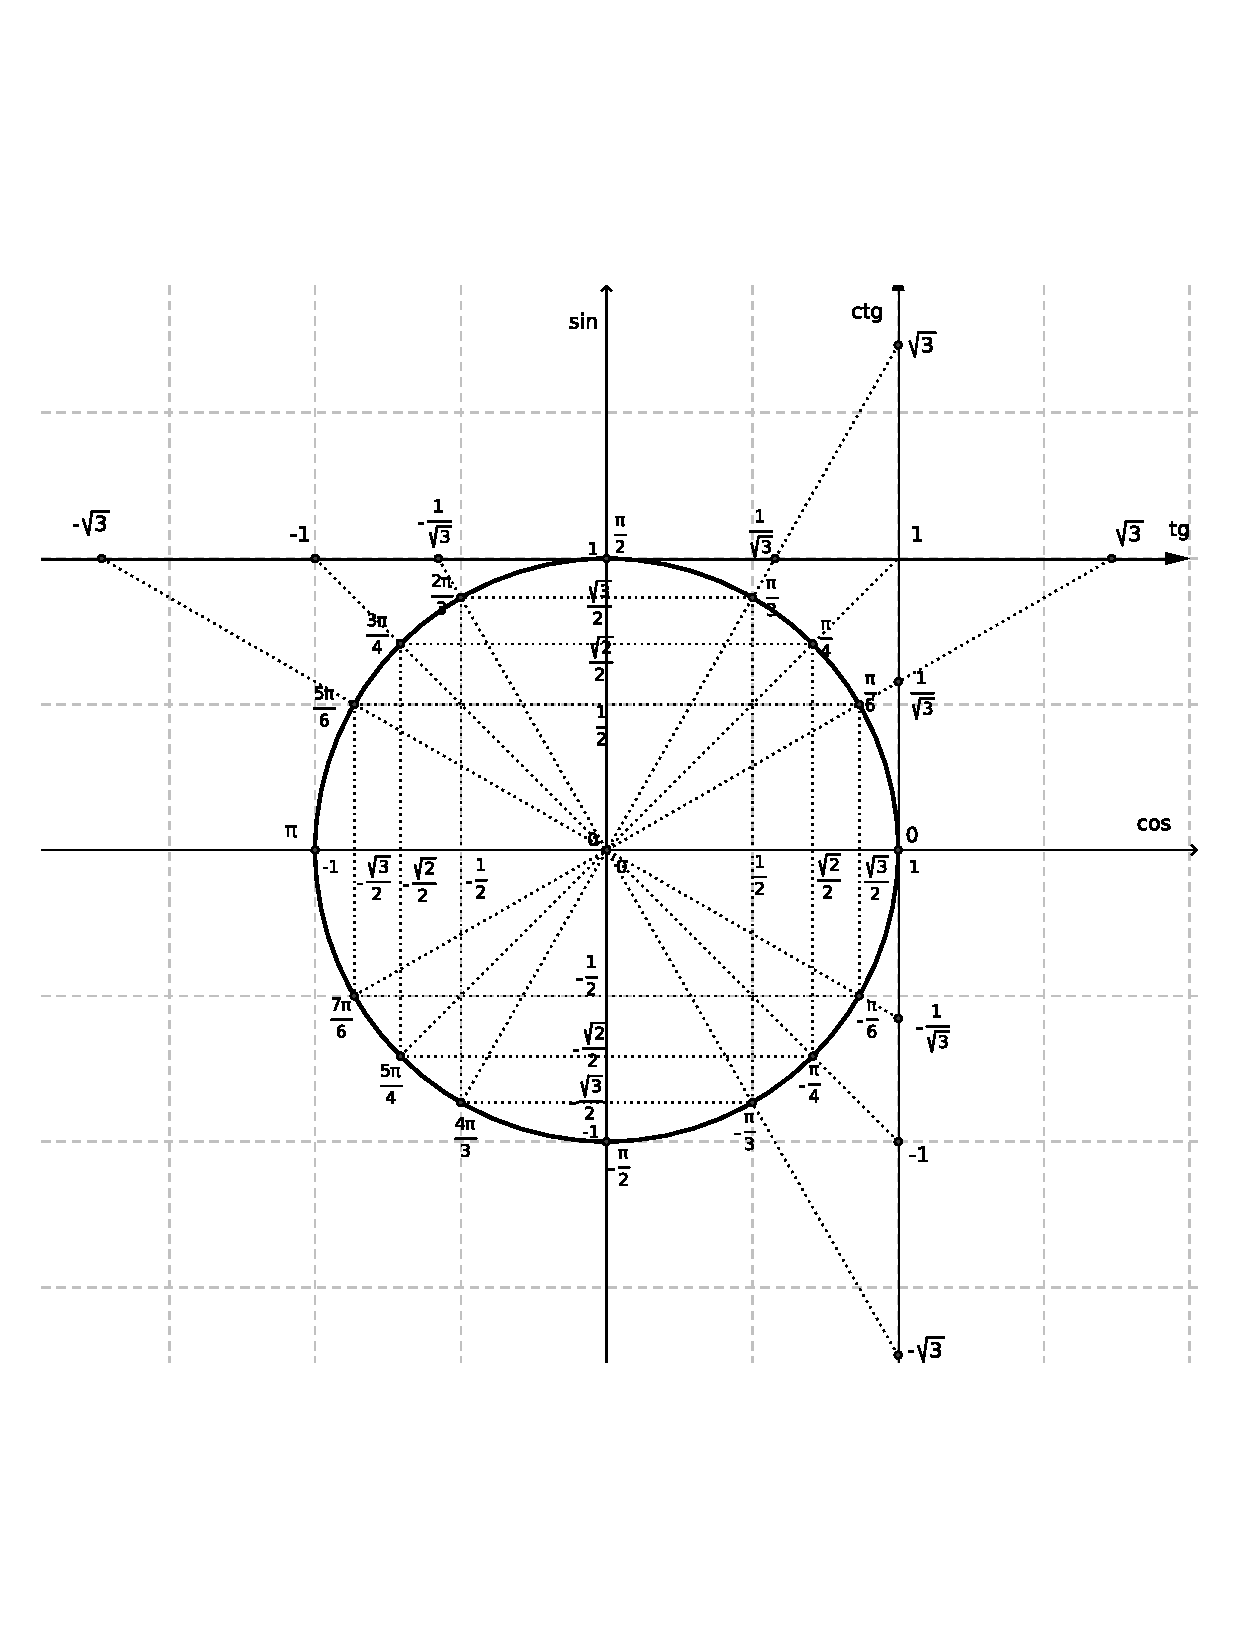
\includegraphics[scale=0.74]{trigokr.pdf}
 % trig.pdf: 1382x1099 pixel, 72dpi, 48.75x38.77 cm, bb=0 0 1382 1099
\end{center}


% \newpage
% 
\section*{������������������ ��������� ���.}
\setcounter{z}{0}

\textbf{�)  ������ ���������.}

\textbf{�) ������� ��� ����� �� ������� ����������. }


\zad   �) $ 2\cos^2 x+\sqrt3\cos x=0$. \quad �) $[-2\pi; -\pi]$.

\zad   �) $\sqrt{2} \sin^2 x=\sin x $. \quad �) $[-2,5\pi; -1,5\pi]$.

\zad   �) $ 3\tg^2x=1$. \quad �) $[0,5\pi; 3\pi]$.

\zad   �) $\cos^2x=1-\sin x $. \quad �) $[2\pi; 3,5\pi]$.

\zad   �) $\sin2x=\sin x $. \quad �) $[-\pi; 1,5\pi]$.

\zad   �) $ \sin x =\cos \dfrac{x}{2}$. \quad �) $[-4\pi; -\pi]$.

\zad   �) $\cos x= \cos \dfrac{x}{2}$. \quad �) $[3\pi; 6\pi]$.

\zad   �) $\cos x=\sin\dfrac{x}{2} $. \quad �) $[\pi; 5\pi]$.

\zad �) $ \dfrac{4\cos^3x-\cos x}{\tg x-\sqrt{3}}=0.$\quad �) $[-3\pi; -\pi]$.

\zad  �) $ 4\cos^2\dfrac{x}{2}-1=\sin x+\sin2x$. \quad �) $[-1,5\pi; 0,5\pi]$.


\zad  �) $ 0,5\sin^2x=\cos(1,5\pi+x)$. \quad �) $[\pi; 3\pi]$.

\zad  �) $6\tg^2x+\dfrac{5}{\cos x}=0$. \quad �) $[-3,5\pi; -0,5\pi]$.

\zad  �) $3\cos2x+13\sin x-9=0$. \quad �) $[0,5\pi; 3\pi]$.

\zad a) ${\cos2x-3\sin2x}=\cos^2 x.$
 \quad
 �)  $[-5\pi; -1,5\pi]$.

\zad  �) $(1+\tg^2 x)\cos\left(\dfrac{\pi}{2}-2x \right)=0 $.
 \quad
 �)  $[1,5\pi; 3\pi]$.

\zad  �) $6\sin x \cos2x+4=8\sin x+3\cos2x$. \quad �) $[-2\pi; \pi]$.

\zad  �) $(2\cos x-1)\sqrt{\sin(x+1,5\pi)}=0$. \quad �) $[2\pi; 5\pi]$.

\zad  �) $ \sqrt{3}\cos x+2\sin^2x+1=0$. \quad �) $[-2\pi; 0]$.

\zad  �) $ \sqrt{3}\sin2x-2=4\sin x-\sqrt{3}\cos x$. \quad �) $[3\pi; 5\pi]$.

\zad  �) $ \sin2x-2\cos^2x=\cos2x$. \quad �) $[13\pi; 15\pi]$.

\zad a)  $(\sin x-\sin 3)(\cos x-\cos 3)=0.$
 \quad
 �)  $[1,5\pi; 2,5\pi]$.

  \zad a)  $\dfrac{4\ctg^2x+3\ctg x}{5\cos^2 x-3\cos x}=0,$\quad  �) $[2\pi;4\pi].$ \\

 \zad a)  $\dfrac{(41\sin^2x-16)(5\tg x+4)}{\sqrt{41}\cos^2 x-5\cos x}=0,$\quad  �) $[2\pi;4\pi].$ \\

 \zad a)  $\dfrac{24\ctg 2x+7}{50\cos^2x-32}=0,$ \quad �) $[7\pi;10\pi].$ \\

 %\zad a)  $\dfrac{(\cos^4x-\sqrt{3}\cos^3x)(\ctg^4x-4)}{(\sqrt{3}\sin^4x-\sin^3x)(4\tg^4x+1)}=0,$\quad  �) $[1,5\pi;2\pi].$ \\


% \zad  �)  $\cos(3x+5)+\sin\left(\dfrac{3\pi}{2}- 2x \right)=0 $.
%  \quad
%  �)  $[-0,5\pi; 1,5\pi]$.
%
%
% \zad  �) $ \log_{\sin x}{\sqrt{3}\cos x}=1$. \quad �) $[-0,5\pi; 2,5\pi]$.
%
% \zad  �) $ \dfrac{\log_7(\sqrt{3}\tg x)}{\sqrt{-7\sin x}}=0$. \quad �) $[-\pi; 1,5\pi]$.
%
% \zad  �) $\dfrac{(\tg x+\sqrt{3})\log_7(2\sin^2x)}{\log_7(\sqrt{2}\cos x)}=0 $. \quad �) $[0; 3\pi]$.
%

% \newpage
% 
\section*{������ ���� �1.}
\setcounter{z}{0}

\textbf{�)  ������ ���������.}

\textbf{�) ������� ��� ����� �� ������� ����������. }


\zad  �) $ 2\sin^2x-3\cos x-3=0$. \quad �) $[\pi; 3\pi]$.


\zad  �) $ \cos 2x+\sin^2x=0,25$. \quad �) $[3\pi; 4,5\pi]$.


\zad  �) $ \dfrac{1}{\tg^2x}-\dfrac{2}{\tg x}-3=0$. \quad �) $[2\pi; 3,5\pi]$.


\zad  �) $\sin^2 x-2\sin x\cdot\cos x-3\cos^2x=0 $. \quad �) $[-\pi; 0,5\pi]$.

\zad  �) $ 3\sin^2x-4\sin x\cos x+5\cos^2x=2.$\quad �) $[-3\pi; -\pi]$.

\zad  �) $ 4\tg x-3\ctg x=1.$\quad �) $[2\pi; 3\pi]$.


\zad  �) $ 36^{\sin2x}=6^{2\sin x}$. \quad �) $[-3,5\pi; -2,5\pi]$.


\zad  �) $ \dfrac{4^{\cos^2\frac{x}{2}}}{(\sqrt{2})^{\sin x}}=\left( 2^{\sin\frac{x}{2}}\right)^{\sin\frac{x}{2}}.$\quad �) $[-1,5\pi; 0,5\pi]$.


\zad  �) $ \sin x\cdot\sin 5x=\cos 4x$. \quad �) $[-2\pi; -0,3\pi]$.

\zad  �) $ \cos x\cdot \cos 5x=\cos 6x$. \quad �) $[-1,2\pi; 0,2\pi]$.


\zad  �) $ \sin 2x+\sqrt{2}\sin x=0$. \quad �) $[-1,5\pi; 1,5\pi]$.


\zad  �) $ 4\sin^3x=3\cos\left( x-\dfrac{\pi}{2}\right)$. \quad �) $[3,5\pi; 4,5\pi]$.


\zad  �) $ 4\cos^2\dfrac{x}{2}-1=\sin x+\sin2x$. \quad �) $[-1,5\pi; 0,5\pi]$.


\zad  �) $ 5\sin^2x=\cos(1,5\pi+x)$. \quad �) $[\pi; 3\pi]$.

\zad  �) $6\tg^2x+\dfrac{5}{\cos x}=0$. \quad �) $[-3,5\pi; -0,5\pi]$.

\zad  �) $3\cos2x+13\sin x-9=0$. \quad �) $[0,5\pi; 3\pi]$.

\zad  �) $6\sin x \cos2x+4=8\sin x+3\cos2x$. \quad �) $[-2\pi; \pi]$.

\zad  �) $(2\cos x-1)\sqrt{\sin(x+1,5\pi)}=0$. \quad �) $[2\pi; 5\pi]$.

\zad  �) $ \sqrt{3}\cos x+2\sin^2x+1=0$. \quad �) $[-2\pi; 0]$.

\zad  �) $ \sqrt{3}\sin2x-2=4\sin x-\sqrt{3}\cos x$. \quad �) $[3\pi; 5\pi]$.

\zad  �) $ \sin2x-2\cos^2x=\cos2x$. \quad �) $[13\pi; 15\pi]$.

\zad  �) $ \tg(x+0,25\pi)+1=2(\sqrt{2}+1)\ctg x$. \quad �) $[-0,25\pi; 1,75\pi]$.

\zad  �) $ \sin\left(2x+\dfrac{\pi}{2} \right)=\cos\left(x+\dfrac{\pi}{2} \right)+\sin\left(x+\dfrac{\pi}{2} \right)$. \quad �) $[-1,5\pi; 3\pi]$.

\zad  �) $ (3\cos x+2)(\sqrt{-\sin x}-1)=0$. \quad �) $[\pi; 5\pi]$.

\zad  �) $ \sqrt{\sin 3x}=\sqrt{1+2\sin4x\cos x}$. \quad �) $[-\pi; 3\pi]$.

\zad  �) $ \sqrt{\cos 2x}=\sqrt{2}\cos(x+\frac{\pi}{2})$. \quad �) $[-1,5\pi; \pi]$.

\zad  �) $ \dfrac{2\sin^2x-\sin(1,5\pi+x)-1}{\sqrt{\sin x}}=0$. \quad �) $[-3\pi; 0]$.

\zad  �) $ \log_{\sin x}{\sqrt{3}\cos x}=1$. \quad �) $[-0,5\pi; 2,5\pi]$.

\zad  �) $ \dfrac{\log_7(\sqrt{3}\tg x)}{\sqrt{-7\sin x}}=0$. \quad �) $[-\pi; 1,5\pi]$.

\zad  �) $\dfrac{(\tg x+\sqrt{3})\log_7(2\sin^2x)}{\log_7(\sqrt{2}\cos x)}=0 $. \quad �) $[0; 3\pi]$.


% \newpage \Large
% 
\section*{����� ��������� � ������������.}
\setcounter{z}{0}

\zad ������� ������� ��������� � ���������� ���������� ���� ������ �������������, ���� ������������

�) ��� � ������ 1;

�) ���������� ����������� ������, ��� ����� ������� ����� 1;

�)  ���������� ������������� ������, ��� ����� ������� ����� 1;

�)  ���������� ��������������� ��������, ��� ����� ������� ����� 1;

�)  ���������� ����������� ��������, ������� ��������� ������� ����� $4\sqrt{3}$, � ������� ����� ����� 5.


\zad  ���� ����� $A(-3;5;4)$ � $B(4;-2;4)$. �������: �) ���������� �������� ������� $AB$; �) ���������� ������� $\overrightarrow{AB}$; �) ����� ������� $AB$;
�) ���������� �����, �������� ������� $AB$ � ��������� $3:4$.


\zad  ���� ����� $A(-8; 13; -7)$ � $B(7;-2;-37)$. �������: �) ���������� �������� ������� $AB$; �) ���������� ������� $\overrightarrow{BA}$; �) ����� ������� $AB$;
�) ���������� �����, �������� ������� $AB$ � ��������� $11:4$.


\zad ����� ���� �����  $A(-3;2;0)$, $B(2;4;-1)$ � $C(7;-3;1)$.     ������� ���������� ����� ����������� ������ ������������ $ABC$.

\zad � ��������� ���� $ABCDA_1B_1C_1D_1$ ��
���������� ������ $AD_1$ � $D_1B_1$ ����� ����� $E$ �
$F$ ���, ��� $D_1E =\dfrac13 AD_1$, $D_1F =\dfrac23 D_1B_1$. �������
����� ������� $EF$.



\zad � ���������� ��������������� ������  $ABCDA_1B_1C_1D_1$ ������� ��������� ����� 2, � ������� ����� ����� 4. �� ������� $A_1B$ �������� ����� $E$ ���, ��� $EC_1=3$. ������� $AE$.


\zad ����������  ������  ������  $ABCA_1B_1C_1$     ��������  ��������������
�����������  $ABC$,  �  �������  $CB=CA=5$, $AB=6$.  ������  ������  �����  24.
�����  $M$  ---  ��������  �����  $AA_1$,  �����  $K$ ����� �����   $B_1C_1$ � ��������� $2:3$ ������ �� ������� $B_1$.  ������� $KM$.


\zad � ��������� ������ ������ $ABCDA_1B_1C_1D_1$ ����� ���������� �������� $ABCD$ � ����������� $AD=20$, $BC=10$ � ������� �������� $AB=13$. ������ ������ ����� 9.
�������  ����������  ��  �����  $C$  ��  ����� ����������� ������ $AC_1$ � $B_1D$.

\zad � ���������� ��������������� �������� $SABCD$ ������ ����� $\sqrt{7}$, � ������� ��������� ����� 6. ������� ���������� �� ����� $A$ �� ����� ����������� ������ ������������ $SBC$.

\zad � ���������� ������������� ������  $ABCDEFA_1B_1C_1D_1E_1F_1$  ������ �����
�����  $2\sqrt{ 3}$. ���������� ���������� ����� ���������� $AB_1$ � $CE$.

% \newpage \Large
% 
\section*{����� ��������� � ������������. ���� ����� ���������.}
\setcounter{z}{0}

\zad ������� ��������� ������������ �������� $\overrightarrow{a}\{2;3;4\}$ � $\overrightarrow{b}\{3;-2;1\}$.

\zad ������� ��������� ������������ �������� $\overrightarrow{a}\{2;3;4\}$ � $\overrightarrow{b}\{3;-2;0\}$.

\zad ������� ���� ����� ��������� $\{1;0;1\}$ � $\{2;2;0\}$.

\zad ������� ���� ����� ��������� $\{1;0;1\}$ � $\{-3;7;3\}$.



\zad � ���� $ABCDA_1B_1C_1D_1$ ������� ����  ����� ������� $A_1D$ � $D_1E$, ��� $E$ --- ��������
  ����� $CC_1$.


\zad    �   ����������      �����������    ������
$ABCA_1 B_1C_1$, ��� ����� ������� ����� 1, �������
������� ���� ����� �������  $AB_1$ � $BC_1$.

\zad �������� ��������� ���������, ���������� ����� ������ ��������� � ���������������� ������� $\{1;2;3\}$.

\zad �������� ��������� ���������, ���������� ����� ����� $P(-2;5;3)$ � ���������������� ������� $\{1;2;3\}$.

\zad ��������� ��������� ���������, ������������ ��������� $6x+3y-z=0$ � ���������� ����� ����� $A(3;-2;1)$.

\zad ������� ���������� ������� ��������� �����, ���������������� ��������� ${x+2y+2z=5}.$

\zad �������� ��������� ���������, ���������� ����� ����� $(3;0;0)$, $(0;4;0)$ � $(0;0;5)$.

\zad �������� ��������� ���������, ���������� ����� ����� $(1;0;2)$, $(2;1;0)$ � $(-1;0;1)$.

\zad �������� ��������� ���������, ���������� ����� ����� $(-1;0;2)$, $(-2;1;0)$ � $(0;1;-2)$.

\zad ������� ���� ����� �����������, ��������� ����������� $x+y+3=0$ � \\${2x+2z-13=0}$.

\zad ������� ���� ����� �����������, ��������� ����������� $3x+2y-z+3=0$ �\\ $6x+4y-2z-13=0$.

\zad ������� ���� �����
   ���������� $9x-12y-20z+14=0$ � �������� $\{2;-1;2 \}$.

\zad ������� ���� �����
   ���������� $-x+y-z+1=0$ � �������� $\{1;-2;0 \}$.


\zad
   � ����  $ABCDA_1B_1C_1D_1$ ������� ���� ����� ����������� $ABC_1$ � $BDD_1$.

\zad
   � ����  $ABCDA_1B_1C_1D_1$  ����� $E$ --- ��������
����� $A_1B_1$. ������� ����� ���� ����� ������
  $AE$ � ���������� $BDD_1$.

 \zad  � ����  $ABCDA_1B_1C_1D_1$  ������� ������� ����
����� ������ $AA_1$ � ���������� $BC_1 D$.

%  \zad  � ������������� ��������������� $ABCDA_1B_1C_1D_1$ ������� ���� �����
%   ���������� $A_1BC$ � ������ $BC_1$, ���� $AA_1=8$, $AB=6$, $BC=15$.


% 
% % \newpage
% % 

\section*{����������� ������.}
\setcounter{z}{0}


\zad 
������� ������������ $ABC$ ����� 12. $DE$ --- ������� �����, ������������ ������� $AB$. ������� ������� �������� $ABDE$.

\smallskip


\zad
������� ���������� �������� ������� $ y~=~4\tg x-4x+\pi -9$ �� ������� $ [-\frac{\pi }{4};\frac{\pi }{4}]$.

\smallskip


\zad  �) ������ ���������  $\dfrac{\sin(x-\frac{\pi}{4})}{\cos x-\frac{\sqrt{2}}{2}}=0.$

�) ������� �����, ������������� ������� $[3\pi; 4,5\pi]$.

\smallskip


\zad ������ �����������  $x^2>4.$

\smallskip

\zad  ������ �����������   
 $\sqrt{x+9}>3-x.$



% 
% \newpage
% 
\section*{���������� �����.}
\setcounter{z}{0}

\Large



\zad (��� 2012) ����� $E$ --- �������� ����� $DD_1$  ���� $ABCDA_1B_1C_1D_1$ ������� ���� ����� �������  $CE$ � $AC_1$.



\zad �    �������������      ���������������
$ABCDA_1B_1C_1D_1$ ������� ���� ����� ����������
$AA_1C$ � ������ $A_1B$, ���� $AA_1 = 3$, $AB = 4 $,
$BC = 4$.

\zad �  �������������  ���������������  $ABCDA_1B_1C_1D_1$    $AB=AA_1=4$, $AD=3$.

�������  �������  ����,  �������  ��������  ���������  $ACB_1$  �  ������ $CDD_1C_1$.


\zad      �    �������������       ���������������
 $ABCDA_1B_1C_1D_1$, � �������� $AA_1= 4 $, $A_1D_1= 6 $,
$C_1D_1= 6$ ������� ������� ���� ����� ���������� $ADD_1$ � ������ $EF$, ���������� ����� �������� ����� $AB$ � $B_1C_1$.


\zad (��� 2012) � ���������� ��������������� ������  $ABCDA_1B_1C_1D_1$ ������� ��������� ����� 2, � ������� ����� ����� 5. �� ����� $AA_1$ �������� ����� $E$ ���, ��� $AE:EA_1=3:2$. ������� ���� ����� ����������� $ABC$ � $BED_1$.


\zad � ������������� ���������������      $ABCDA_1B_1C_1D_1$ �������� ����� �����: $AA_1= 5$,
 $AB = 12$, $AD = 8$. ������� ������� ���� �����
���������� $ABC$ � ����������, ����������
����� ����� $B$ ��������������� ������ $AK$,
���� $K$ --- �������� ����� $C_1D_1$.









\zad
 � ���������� ����������� ������
 $ABCA_1B_1C_1$, ��� ����� ������� ����� 1, �������
���� ����� ����������� $ACB_1$ � $A_1C_1B$.


%\zad      � ���������� ����������� ������
%$ABCA_1B_1C_1$, ��� ����� ������� ����� 1, ����� $D$,
%$E$ --- �������� ����� �������������� $A_1B_1$ � $A_1C_1$.
%������� ������� ���� ����� ����������� $ADE$
%� $BCC_1$.


\zad  � ���������� ����������� ������
$ABCA_1B_1C_1$, ��� ����� ������� ����� 1, �������
���� ����� ������ $AB_1$ � ���������� $AA_1C_1C$.


\zad � ���������� ������������� ������ $ABCDEFA_1B_1C_1D_1E_1F_1$ ��� ����� ����� 1. ������� ������� ���� ����� �������
 �) $AB_1$ � $BC_1$; �) $AB_1$ � $BD_1$.

\hans{\dfrac{\sqrt{2}}{4}}

\zad      � ���������� ������������� ������
$ABCDEFA_1B_1C_1 D_1 E_1 F_1$, ��� ����� ������� �����
1, ����� $G$ --- �������� ����� $A_1B_1$. ������� ���� �����:

�) ������ $AG$ � ���������� $BCC_1$;

�) ������ $FG$ � ���������� $ACD_1$.

\zad ����������  ������  ������  $ABCA_1B_1C_1$     ��������  ��������������
�����������  $ABC$,  �  �������  $AB=AC=10$,  $BC=16$.  ������  ������  �����  3.
����� $M$ --- �������� ����� $A_1B_1$. ������� ������� ���� ����� ������ $MB$
� ���������� $BCC_1$.


\zad            � ���������� ��������������� �������� $SABCD$, ��� ����� ������� ����� 1,
������� ���������� ���� $ABSC$.



\zad (��� 2010) � ���������� ����������� �������� $SABC$ � ���������� $ABC$ �������� �����: $AB=12\sqrt{3}$, $SC=13$. ������� ����, ������������ ����������
��������� � ������ $AM$, ��� $M$ --- ����� ����������� ������ ����� $SBC$.



%
%\zad    � ���������� ������������� ��������
%$SABCDEF$, ������� ����� ������� ����� 2, �
%������� ��������� --- 1, ������� ����
%����� ������ $AC$ � ���������� $SAF$.
%
%
%
%
%\zad ���������� ������ ����������� ������ $ABCA_1B_1C_1$ �������� �������������� ����������� $ABC$, � ������� $AB=BC=20$, $AC=32$. ������� �����
%������ ����� 24. ����� $P$ ����������� ����� $BB_1$, ������ $BP:PB_1=1:3$. ������� ������� ���� ����� ����������� $A_1B_1C_1$ � $ACP$.
%
%\hans{ }
%
%\zad ���������� ������ ����������� ������ $ABCA_1B_1C_1$ �������� �������������� ����������� $ABC$, � ������� $AB=AC=8$, � ����
%�� ����� ����� $60{}^{\circ}$. ����� $P$ ����������� ����� $AA_1$, ������ $AP:PA_1=2:1$. ������� ������� ���� ����� �����������
% $A_1B_1C_1$ � $BCP$, ���� ���������� ����� ������� $AB$ � $C_1B_1$ ����� $18\sqrt{3}.$
%
%\hans{ }
%
%
%
%\zad ���������� ������ ����������� ������ $ABCA_1B_1C_1$ �������� �������������� ����������� $ABC$, � ������� $AB=AC=5$, � $BC=8$. ������ ������ ����� 3. ������� ���� ����� ������ $A_1B$ �  ���������� $BCC_1$.
%
%\hans{\arctg 0,6 } 
% 
% \newpage
% \onecolumn
\section*{������ ������ C2 ���. ����������.}
\setcounter{z}{0}

{\bf ���������� �� ����� �� ������}

\zad � ��������� ���� $ABCDA_1B_1C_1D_1$ ������� ���������� �� ����� $A$ �� ������:\\
 a) $B_1D_1$; \, �) $BD_1$.

\zad  � ���������� ������������� ������
$ABCDEFA_1B_1C_1 D_1 E_1 F_1$, ��� ����� ������� �����
1, ������� ���������� �� ����� $A$ �� ������:\\
a) $DE$;
�) $D_1E_1$;
�) $B_1C_1$;
�) $BE_1$;
�) $BC_1$;
�) $CE_1$;
�) $CF_1$;
�) $CB_1$.

\zad � ��������� $ABCD$, ��� ����� �������� ����� l ,
����� ���������� �� ����� $A$ �� ������, ���������� ����� ����� $B$ � �������� $E$ ����� $CD$.

{\bf ���������� �� ����� �� ���������}

\zad � ��������� ���� $ABCDA_1B_1C_1D_1$ ������� ���������� �� ����� $A$ ��
��������� $A_1BC_1$.

\zad ��� ��� $ABCDA_1B_1C_1D_1$. ����� ����� ���� ����� 1. �������
���������� �� �������� ������� $BC_1$ �� ��������� $AB_1D_1$.



\zad  � ���������� ������������� ������
$ABCDEFA_1B_1C_1 D_1 E_1 F_1$, ��� ����� ������� �����
1, ������� ���������� �� ����� $A$ �� ���������:\\
a) $BCC_1$;
\,
�) $BDC_1$; \,
�) $B_1C_1F$;
\,
�) $BE_1F$; \,
�) $A_1B_1C$. \,


\zad ������� ������ ����������� ��������� � ������ $\sqrt{6}$.


\zad  ����� $AD$ �������� $DABC$ ��������������� ��������� ��������� $ABC$. ������� ���������� �� ������� $A$ �� ���������, ����������
����� �������� ����� $AB$, $AC$ � $AD$, ����
$AD = 2\sqrt{5}$, $AB = AC = 10$, $BC = 4 \sqrt{5}$.



{\bf ���������� ����� �������}




\zad  � ���������� ��������������� �������� $SABCD$, ��� ����� ������� ����� 1,
������� ���������� ����� ������� $BD$ � $SA$.



\zad  � �������� $DABC$ �������� ����� �����:
$AB = AC = DB = DC = 10$, $BC = DA = 12$. ������� ���������� ����� ������� $DA$ � $BC$.



\zad
   � ����  $ABCDA_1B_1C_1D_1$ � ������ 2 ����� $E$ � $F$ --- ��������
����� $A_1B_1$ � $B_1C_1$. ������� ���������� ����� �������:\\
�)   $AE$ � $BF$;
\quad
�)   $AF$ � $BE$;
\quad
�)   $CE$ � $D_1F$.




\zad � ����������� �������� $DABC$ ��� ������� ���� ��� ������� $D$ ������, ������ $AD=16$, $BD=12$, $CD=24$. ����� $K$ � $M$ �������� ����� $AB$ � $CD$ ��������������.
������� ���������� ����� ������� $BM$ � $CK$.

\zad ������� ��������� $ABC$ ���������� ����������� �������� $ABCD$ ����� $8\sqrt{3}$, ������ �������� $DO=6$. ����� $A_1$ � $C_1$ --- �������� ����� $AD$ � $CD$ ��������������. ������� ���������� ����� ������� $BA_1$ � $AC_1$.


\textbf{������}

\zad � ���������� ��������������� �������� $SABCD$ ����� ������� ��������� $AB=3\sqrt{2}$, � ������� ����� ����� 5. ������� ����� $SAD$ ������������ � ����� $M$. ������� ���������� �����:

�) $M$ � $AC$;
\quad
�) $M$ � $BCS$;
\quad
�)$M$ � $ABS$;
\quad
�) $BM$ � $CS$;
\quad
�) $BM$ � $DS$.

\enlargethispage{5mm}
\zad � ����������� �������� $SABC$ � ��������� ����� ���������� ����������� $ABC$ � ������ ������� $AB=6\sqrt{3}$. ��������� $SAB$ ��������� � ��������� ��� ����� $45^{\circ}$, � ������� �����
$SC$ ��������������� ��������� ���������. ����� $M$ � $K$ �������� ����� $SA$ � $SB$ ��������������. �������
a) ���������� �� ������� $A$ �� ��������� $CMK$;
\quad
�) ���������� ����� ������� $AK$ � $CM$.


% \newpage \Large
% \onecolumn
\section*{ ������� �������.}
\setcounter{z}{0}

\zad (���2012) ����� $E$ --- �������� ����� $AA_1$ ���� $ABCDA_1B_1C_1D_1$.  ������� �������
������� ���� ���������� $C_1DE$, ���� ���� ���� ����� 2.

\zad ����� ���� $ABCDA_1B_1C_1D_1$ ����� 4.  ������� �������
������� ���� ����������, ���������� ����� �������� ����� $AB$, $AD$ � $B_1C_1$.


\zad ����� ���� $ABCDA_1B_1C_1D_1$ ����� 3. �� ����� $AB$ ����� ����� $M$ ���, ��� $AM:MB=1:2$  ������� �������
������� ���� ����������, ���������� ����� ����� $M$, $B_1$ �  �������� ����� $AD$.

\zad ����� �������� ��������� ���� ��������� ��������� ��������������� ���� ���������. ����� ��������� ������� ������� ���� ������ ���������� � ������� ������ ����������� ����.

\zad � ���������� ��������������� ������  $ABCDA_1B_1C_1D_1$ ������� ��������� ����� 2, � ������� ����� ����� 5. �� ����� $AA_1$ �������� ����� $E$ ���, ��� $AE:EA_1=3:2$. ������� ������� ������� ������ ���������� $BED_1$.

\zad  � ���������� ����������� ������
$ABCA_1B_1C_1$, ��� ����� ������� ����� 1, ����� $D$,
$E$ --- �������� ����� �������������� $A_1B_1$ � $A_1C_1$.
������� ������� ������������ $ADE$.


\zad � ���������� ������������� ������
$ABCDEFA_1B_1C_1 D_1 E_1 F_1$ ��� ����� ����� 2. ������� ������� ������� ������ ���������� $ABC_1$.



\zad � ���������� ������������� ������
$ABCDEFA_1B_1C_1 D_1 E_1 F_1$ ��� ����� ����� 2. ������� ������� ������� ������ ���������� $ABD_1$.

\zad � �������� $DABC$ �������� ����� �����:
$AB = AC = DB = DC = 10$, $BC = DA = 8\sqrt{2}$. ������� ������� ������� �������� ����������, ���������� ����� ����� $A$, $D$ � �������� $BC$.

\zad (��� 2013) � ���������� ����������� �������� $MABC$ � �������� $M$ ������ ����� 3, � ������� ����� ����� 6. ������� ������� ������� ���� �������� ����������, ���������� ����� �������� ������ $AB$ � $AC$ ����������� ������ $MA$.

\zad (��� 2013) � ���������� �������������� �������� $MABCD$ � �������� $M$ �������
��������� ����� 3, � ������� ���� ����� 8. ������� ������� �������
�������� ����������, ���������� ����� ����� $B$ � �������� ����� $MD$
����������� ������ $AC$.

\zad ����� �������� ������ ���������� ��������������� �������� ��������� �������, ���������������� �������� �����. ������� ������� ����� �������, ���� ����� �������� ����� ����� 4, � ���� ����� �������� �������, �������� � ����� �����, ����� $60^\g$.

\zad � ���������� ����������� �������� $SABC$ � ���������� $ABC$ �������� �����: $AB=12\sqrt{3}$, $SC=12\sqrt{10}$.  $M$ --- ����� ����������� ������ ����� $SBC$. ������� ������� ������� �������� ����������, ���������� ����� ������ $AM$ ����������� ������ $BC$.

\zad (��� 2013) ��������� $\alpha$ ���������� ��� ����, ������� ����� �����. ������� ������� �������� ���� ���� ���������� ����� 7. ��������� $\beta$, ������������ ��������� $\alpha$, �������� �������� ����, � ������� ������� ���� ���������� �������� ���� ����� 5. ������� ������� ������� �������� ���� ���������� $\alpha$.

\zad (��� 2013) ��� ������������ ���������, ���������� ����� �������� 2, ���������� ���. ���� �� ���������� �������� ����� ����� ����.
��������� �������� ������� ���� ����� ����������� ����� 0,84. ������� ������ ����.

\zad (��� 2013) ������ ��������� ������ ����� 8, � ��� ������ ����� 15. ��������� ������� �������� ������� ������ � ����� ���������, ����� ������� ����� 14.
������� ���������� �� ������ ��������� ������ �� ��������� �������.


\zad � ���������� ��������������� �������� $SABCD$ � �������� $S$ ������� ������� ����� $6\sqrt{7}$, � ������� ��������� $6\sqrt{6}$. ����� $M$ � $K$ --- �������� ����� $AD$ � $AB$ ��������������. ����� $E$ ����� �� ����� $SC$. ���� ����� ���������� $MKE$ � ���������� ��������� ����� $30^\g$ ��������. ����� ������� �������, ����������� ����� ����� $M$, $K$ � $E$.

\zad � ���������� ��������������� �������� $SABCD$ � �������� $S$, ����� $M$ --- �������� ����� $BS$. ������� ��������� �������� ����� $6\sqrt{2}$, � ������ �������� ����� 9. ����� ������� �������, ������������ ����� ������ $AM$ ����������� $BD$.


\zad � ��������� ������ ������ $ABCA_1B_1C_1$  ����� ������������� ����������� � ������ ����� $A$, ������ $30^\g$ ��������. ����� ������� ������� ������, ����������� ����� ������� ����� ������� ��������� � �������� ���������� �������� ���������, ���� ���������� ����� ����������� ������ ����� ���������� �� ������� $A$ �� �������� ������� � ����� 6.


\zad � ���������� ����������� ������ $ABCA_1B_1C_1$ �� �������� ��������� ������ $1+\sqrt{3}$ � ������� ������ 2 ��������� ������� ����� ������ $BC$, ������� ����� ������ �� 2 ������������� ������ �������. ����� ������� ����� �������.


\zad � ���������� ������������� ��������
$SABCDEF$, ������� ����� ����� 2, �
������� ��������� --- 1. ������� ������� ������� �������� ����������, ���������� ����� ����� $B$, $C$ � �������� ����� $SE$.

\zad � ��������� ������ ������ $ABCA_1B_1C_1$ ����� ��������������
����������� $ABC$, � �������� ���������
$BC$ ����� 3. ������� ����������� ������ ����� 32. ����� ������� �������
������ ����������, ���������� �����
$CB_1$ ����������� ������ ��������� $AD$,
���� ��������, ��� ���������� �� ����� $A$ �� ��������� ������� ����� 1,2.


%
%
%\zad � ��������� ���� $ABCDA_1B_1C_1D_1$ ������� ���������� �� ����� $A$ �� ������:\\
% a) $B_1D_1$; \, �) $BD_1$.
%
%\zad  � ���������� ������������� ������
%$ABCDEFA_1B_1C_1 D_1 E_1 F_1$, ��� ����� ������� �����
%1, ������� ���������� �� ����� $A$ �� ������:\\
%a) $DE$;
%�) $D_1E_1$;
%�) $B_1C_1$;
%�) $BE_1$;
%�) $BC_1$;
%�) $CE_1$;
%�) $CF_1$;
%�) $CB_1$.
%
%\zad � ��������� $ABCD$, ��� ����� �������� ����� l ,
%����� ���������� �� ����� $A$ �� ������, ���������� ����� ����� $B$ � �������� $E$ ����� $CD$.
%
%
%
%\zad � ��������� ���� $ABCDA_1B_1C_1D_1$ ������� ���������� �� ����� $A$ ��
%��������� $A_1BC_1$.
%
%\zad ��� ��� $ABCDA_1B_1C_1D_1$. ����� ����� ���� ����� 1. �������
%���������� �� �������� ������� $BC_1$ �� ��������� $AB_1D_1$.
%
%
%
%\zad  � ���������� ������������� ������
%$ABCDEFA_1B_1C_1 D_1 E_1 F_1$, ��� ����� ������� �����
%1, ������� ���������� �� ����� $A$ �� ���������:\\
%a) $BCC_1$;
%\,
%�) $BDC_1$; \,
%�) $B_1C_1F$;
%\,
%�) $BE_1F$; \,
%�) $A_1B_1C$. \,
%
%
%\zad ������� ������ ����������� ��������� � ������ 6.
%
%
%\zad  ����� $AD$ �������� $DABC$ ��������������� ��������� ��������� $ABC$. ������� ���������� �� ������� $A$ �� ���������, ����������
%����� �������� ����� $AB$, $AC$ � $AD$, ����
%$AD = 2\sqrt{5}$, $AB = AC = 10$, $BC = 4 \sqrt{5}$.
%
%
%
%
%\zad  � ���������� ��������������� �������� $SABCD$, ��� ����� ������� ����� 1,
%������� ���������� ����� ������� $BD$ � $SA$.
%
%
%
%\zad  � �������� $DABC$ �������� ����� �����:
%$AB = AC = DB = DC = 10$, $BC = DA = 12$. ������� ���������� ����� ������� $DA$ � $BC$.
%
%
%
%\zad
%   � ����  $ABCDA_1B_1C_1D_1$ � ������ 2 ����� $E$ � $F$ --- ��������
%����� $A_1B_1$ � $B_1C_1$. ������� ���������� ����� �������:\\
%�)   $AE$ � $BF$;
%\quad
%�)   $AF$ � $BE$;
%\quad
%�)   $CE$ � $D_1F$.
%
%
%
%
%\zad � ����������� �������� $DABC$ ��� ������� ���� ��� ������� $D$ ������, ������ $AD=16$, $BD=12$, $CD=24$. ����� $K$ � $M$ �������� ����� $AB$ � $CD$ ��������������.
%������� ���������� ����� ������� $BM$ � $CK$.
%
%\zad ������� ��������� $ABC$ ���������� ����������� �������� $ABCD$ ����� $8\sqrt{3}$, ������ �������� $DO=6$. ����� $A_1$ � $C_1$ --- �������� ����� $AD$ � $CD$ ��������������. ������� ���������� ����� ������� $BA_1$ � $AC_1$.
%
%
%\textbf{������}
%
%\zad � ���������� ��������������� �������� $SABCD$ ����� ������� ��������� $AB=3\sqrt{2}$, � ������� ����� ����� 5. ������� ����� $SAD$ ������������ � ����� $M$. ������� ���������� �����:
%
%�) $M$ � $AC$;
%\quad
%�) $M$ � $BCS$;
%\quad
%�)$M$ � $ABS$;
%\quad
%�) $BM$ � $CS$;
%\quad
%�) $BM$ � $DS$.
%
%\enlargethispage{5mm}
%\zad � ����������� �������� $SABC$ � ��������� ����� ���������� ����������� $ABC$ � ������ ������� $AB=6\sqrt{3}$. ��������� $SAB$ ��������� � ��������� ��� ����� $45^{\circ}$, � ������� �����
%$SC$ ��������������� ��������� ���������. ����� $M$ � $K$ �������� ����� $SA$ � $SB$ ��������������. �������
%a) ���������� �� ������� $A$ �� ��������� $CMK$;
%\quad
%�) ���������� ����� ������� $AK$ � $CM$.
%

% 
% \newpage
% 
\section*{������.}
\setcounter{z}{0}

\Large


\zad  ���������� ����������� ������ ������� � ��� ������� $\sqrt{7}$. ����� ����� ������, ���� ��� �� ����� ���������� �����.

 %\emph{�����:} $18.$


\zad  � ��������� ������� ��������������� ����� �������������� �� ��������� 1 � 4 � ������ ����� $60^{\circ}.$ ������� ��������� ��������������� ����� 5. ���������� ��� �����.

 %\emph{�����:} $4\sqrt{3}.$

\zad  � ��������� ���������� ����������� ������ $ABCA_1B_1C_1$ � �������� ������� $AA_1,\;BB_1,\;CC_1$ ����� �������������� ����������� $ABC$ �� �������� 4. ����� ����� ������, ���� ��������, ��� ������ $AB_1$ � $CA_1$ ���������������.

 %\emph{�����:} $8\sqrt{6}.$

\zad  ����� $K$ �������� ��������� ����� $AA_1$ ���������� ����������� ������ $ABCA_1B_1C_1$. �� ������� ����� $CC_1B_1B$ ����� ����� $L$, � �� ��������� $ABC$ --- ����� $M$ ���, ��� ������ $A_1L$ � $KM$ �����������. ����� ���������� ����� ����� ����� ������ $ABCA_1B_1C_1$, ���� $A_1L=1,\;KM=\dfrac{3}{5},\;ML=\dfrac{1}{\sqrt{10}}$?

 %\emph{�����:} $\dfrac{\sqrt{6}}{10}.$

\zad  � ��������� �������� ����� ������������� ����������� � �������� 3 � 4. ��� ������� ����� ��������� � ��������� ��������� ��� ����� �����, ������� �������� ����� 0,8. ������� ����� ��������.

 %\emph{�����:} 4.

\zad  ����������� ���������� ��������� �������� ������ ��������, ��������� ������� ����� 8 � 5. ������� ����� ��������� � ��������� ��������� ��� ����� $45^{\circ}$. ���������� ����� ��������� ��������.

 %\emph{�����:} 32,25.

\zad  ���� ����� ������� ������ � ���������� ��������� ���������� ����������� �������� ����� $45^{\circ}$. ����� �������� ����� $\dfrac{1}{3}$. ����� ����� ������� ��������� ��������.

 %\emph{�����:} 2.


\zad  ���������� �������� ������ � ����� ������� $3\sqrt{3}$. ����� ����� ���������.

 %\emph{�����:} 72.

\zad  � ��������� �������� ����� �������������� ����������� � ���������� 6 � ������� 9. ������ ������� ����� ����� 13. ��������� ����� ��������.

 %\emph{�����:} 108.

\zad  ��� ������� 0,5 ������ � ��������, � ��������� ������� ����� ���� � ����� $30^{\circ}$. ������� ����� ��������� � ��������� ��������� ��� ����� $60^{\circ}$. ����� ����� ��������.

 %\emph{�����:} 3.

\zad  ����� ��������� $BD$ ��������� ���������� ��������������� �������� $ABCDE$ ��������� ������� $BDK$ ��� ����� $45^{\circ}$ � ��������� ���������. ����� $K$ ����� ������� ����� $AE$ �������. ����� ����� �������� $ABDK$, ���� ����� $AE=15\sqrt{2}$.

 %\emph{�����:} 562,5.

\zad  ����� ������ �����, ��������� ����� ���������� ����������� ��������, ���� �� ����� ����� $\dfrac{3\sqrt{3}}{2}$, � ������ 2.

 %\emph{�����:} 1,75

\zad  ������� ���������� �������� ������ �������� $ABCD$, ��������� � ����� c ��������� $AB=4$.

%\emph{�����:} $\dfrac{8}{3}.$


\zad  � ���������� ����������� �������� $ABCD$ ����� ������� ��������� $BC$ ��� ����� $30^{\circ}$ � ��������� ��������� $ABC$ ��������� ������� $BCK$. ����� $K$ ����� ����� $AD$ ���, ��� $AK:KD=1:2$. ����� ����� �������� $ABCK$, ���� ������� ��������� $AB=6\sqrt{3}.$

 %\emph{�����:} 63.

% 
% \newpage
% 
\section*{���������� �2.}
\setcounter{z}{0}



\zad �    �������������      ���������������
$ABCDA_1B_1C_1D_1$ �������� ����� $AA_1 = 12$, $AB = 3 $,
$BC = 4$.
  �����  ��������  �����  $AB$  ���������������  ���������  $BD_1$
���������  ���������.  �������  ����,  ������������  ����  ����������  �
���������� ���������������.


\zad �������
���������
����������
�������������
������
$ABCDEFA_1B_1C_1D_1E_1F_1$   �����  12,  �  ������  �����  9.  �������  ����������  ��
����� $A$ �� ���������  $(A_1FD)$.

\zad ����������  ������  ������  $ABCA_1B_1C_1$     ��������  ��������������
�����������  $ABC$,  �  �������  $CB=CA=5$, $AB=6$.  ������  ������  �����  24.
�����  $M$  ---  ��������  �����  $AA_1$,  �����  $K$ ---  ��������  ����� $BB_1$.  �������
���� ����� ���������� $MKC_1$ � ���������� ��������� ������.


\zad � ��������� ������ ������ $ABCDA_1B_1C_1D_1$ ����� ���������� �������� $ABCD$ � ����������� $AD=20$, $BC=10$ � ������� �������� $AB=13$. ������ ������ ����� 9.
�������  ����������  ��  �����  $C$  ��  ��������� $ADC_1$.

\zad � ���������� ��������������� �������� ������ ����� $\sqrt{7}$, � ������� ��������� ����� 6. ������� ���� ����� �����������, ����������� ��� �������� ������� ����� ���� ��������.

\zad � ���������� ������������� ������  $ABCDEFA_1B_1C_1D_1E_1F_1$  ������ �����
�����  $2\sqrt{ 3}$. ���������� ���������� ����� ������� $AD_1$ � $CB_1$.

\zad  � �������� �������, ������������ ���������, ����� ������ � ��������� 2:3 ������ �� �������. ����� ������� �������, ����, ��� ��� ������ ������� ��������� �� 84.

 %\emph{�����:} 16.

\zad  � ���� $ABCDA_1B_1C_1D_1$ ����� ������� $A,\;C_1$ � ��������
����� $D_1D$ ��������� �������. ����� ����� ����, ���� �������
������� ����� $50\sqrt{6}.$

 %\emph{�����:} $10.

\zad  � ���������� ��������������� �������� ������� ��������� ����� 8, � ���� ������� �������� ����� � ��������� ��������� ����� $60^{\circ}$. ����� ������� ������� �������� ����������, ���������� ����� ������� ��������� ��������������� ��������������� �����.

%\emph{�����:} $\dfrac{100\sqrt{3}}{3}.$

\zad  � ���������� ��������������� �������� ������� ��������� ����� 8, � ���� ������� �������� ����� � ��������� ��������� ����� $60^{\circ}$. ����� ������� ��������� ����������� �������������� �� ��������� ��������� ������� ��������� ���, ��� ������ �������� ������� ������ ����������� � ���� ���������� � ��������� $1:2$ ������ �� ���������. ����� ������� �������.

 %\emph{�����:} $\dfrac{64\sqrt{3}}{3}.$


\zad  ������ ����� ��������� $ABCD$ ����� ����� $3\sqrt{2}$. ��
����� $AD$ ������� ����� $M$ ���, ��� ${AM:MD=2:1}$. ���������
������� ������� ��������� ����������, ����������� ����� ����� $M$
��������������� ����� $AD$.

 %\emph{�����:} 2.

% 
% 
% \newpage
 
\section*{��������� ������.}
\setcounter{z}{0}

\zad
��������� �������� ������� � 2000 ���� ������� � ������� 1000000 ������. ������ ��������� ��� ��� ������� ������������� �� 7\% �� ��������� � ���������� �����. ������� ������ ��������� �������� �� 2002 ���?

\zad
������� 9 ������ 40-����������� ������� �������� ���������� �������� � 11 ������� 20-����������� ������� �������� ����� �� ��������. ������� ��������� ���������� ������������ ������������� ��������?

\zad   ������� ������ ���� ����� ����� �� ���� ����� 80\% ��������
��������, ����� �������� 8\% �����?

\emph{�����: } $9$.


\zad   ������� ��� ������, ���������� 4 � 6 �� �������� �������
������ ������������. ���� �� ����� ������, �� ��������� �������,
���������� 35\% �������. ���� �� ����� ������ ����� ����
���������, �� ��������� �������, ���������� 36\% �������. �������
����������� ������� ���������� � ������ ������?

\emph{�����: } $1,64$ � $1,86$ ��.

\zad    � ������ ���� 12 � ������� �������. ����� ������� ������,
� ����� ������ �����. ����� ����� ������ ������� �� � ����� ������
�����. ������� �������� �������� ������ ���, ���� � ������
�������� 25\% ������� �������?

\emph{�����: } $6$ �.

\zad    ��������� ����� ��������� ����� �� ������ ���������� 18\%.
�� ����� ��������� ��-�� ������ ��������� ����� ���������� �� 2\%.
������� ����� ����������� �����, ���� �� ������ ���� ����������
400 ��.

\emph{�����: } $410$ ��.

\zad    �������� �������� �������� �����. �� ����� 40\% ����
����������. ��� ���� ����� ������� ���������� �� 60\%. ����� �����
(� ���������) ������ ��������� �������� ���� � ����� ������?

\emph{�����: } 36\%.

\zad
����� ������� �� ����, ���� � �� ������ ���������. ���� �� �������� ���� ����������� �����, ����� ����� ����� ����� �� �� 108\%. ���� �� ��������� ������ ����������� �����, ����� ����� ����� ���������� �� �� 2\%. ������� ��������� �� ������ ������ ����� ���������� �������� ����?

\emph{�����: } 43\%.

\zad    �������� �������� �� $p$\%. ����� ����� �������� ��������
�� $2p$\%. � ���������� ���� ��������� �������� ����������� � 1,32
����. �� ������� ��������� �������� ���� �������� �� ������ ���?

\emph{�����: } $20$\%.

\zad    � ����� ���� 200 � 80\%~-���� ������. �������� ����� ��
����� ��������� ���������� ����� ������ � ����� ������� � ���
������� �� ����, ����� �������� 60\%~- ��� �����. ������� �������
���� ������� ��������?

\emph{�����: } $50$.

\zad    ������ ����� �������� 92\% ����, � ����� --- 8\%. �������
��������� ����� ������ �� 23 �� ������?

\emph{�����: } $2$.

\zad    ����� ������ ���� � ������ ������ 15 �� �������� 20\%
����. ������� ������ ���� ���������� �������� � ����� ������,
����� ����� ����� �������� 40\% �����?

\emph{�����: } $15$.

\zad
������ ����� �������� 5\% ����, ������  -- 13\% ����. ����� ������� ������ ������ ����� ������� �� 3 ��. 
�� ���� ���� ������� �������� ������ �����, ���������� 12\% ����. ������� ����� �������� ������. ����� ����� � �����������.

\emph{�����: } 4.

\zad    ������� ��� ������ ������ ������ � �����. ������ ������
�������� 230 � ������ � 20 � ����, � ������ ������ --- 240 �
������ � 60 � ����. �� ������� ������ ����� �� �����, �������� ��
� �������� 300 � ������, � ������� ��������� 84\% ������.
���������� ����� (� �������) �����, ������� �� ������� ������.

\emph{�����: } $100$.


\zad    ������ --- ����� ���� � �����. ����� ������ �������� ����
�� 60 �� ������, ��� �����. ���� ����� ������ �������� �� 100 ��
���� � �������� ������, � ������� 70\% ����. ���������� �������
���������� ���� � �������������� ����� ������.

\emph{�����: } $60$.

\zad   ������� ��� ������, � ����� �� ������� ���������� 20\%, � �
������ 30\% �����. ������� ����� ����� ������� � ������� �������,
����� ��������� �� ��� 10 �� ������ ������, ����������� 27\%
�����?

\emph{�����: } $3$ � $7$ ��.


\zad    ������� ��� ������ ������� ������ � ����. � ������ ������
��������� ������ � ���� $1:2$, � �� ������ --- $2:3$. ����
�������� 1/3 ������� ������ � 5/6 �������, �� � ������������
������ ������ �������� �������, ������� � ������ ������ ���� ����.
���� 2/3 ������� ������ �������� � ��������� �������, �� �
������������ ������ �������� ���� �� 1 �� ������, ��� ���� ������
�� ������ ������. ������� ������ ���� � ������ ������?

\emph{�����: } $1,2$ � $2,4$ ��.

\zad    ������� ��� �����, ������������ �� ��������� $A$, $B$ �
$C$. � ������ ����� ������ ������ �������� $A$ � $B$ � �������
��������� $3:5$, �� ������ ����� ������ ������ �������� $B$ � $C$
� ������� ��������� $1:2$, � ������ ����� ������ ������ ��������
$A$ � $C$ � ������� ��������� $2:3$. � ����� ��������� ���� �����
��� �����, ����� �� ����� ���������� ����� �������� $A$, $B$ � $C$
����������� � ������� ��������� $3:5:2$?

\emph{�����: } $20:6:3$.



\zad  � ������� 2000 ���� ������ �� ��������� � ����� ������������ ��������� $x$\% �������, ����� ��� � ������� 2001 ���� --- $y$\% �������,
������ ��������, ��� $x+y=30\%$. � ������� 2000 ���� �������� ������ ���� � ����� ������������, ������� �� ���� ��������� �����.
� ������� 2001 ����, �� ���������� ���� � ���� ��������, �������� ���� �� ����� ����� ����� ���� �����. ������� �������� $x$
��� ������� ����� �� ����� ��������� � ������� 2002 ���� ������ ������������ ���������.

\emph{�����: } 25


\zad   ���� ��� ������������� ������� ������ ��������� �����. ����� ��� �������� ������������ ����� ���� ����� �� �����.
���� �������� ������� ������� �� 40 �������. � ����� ����������� ���� ������������ ����� � 1,44 ���� ���������� ��������������� �����. ����� ������� ����� �������?

\emph{�����: } 60



\zad   ����c������������� �������� Amako Inc. ������ �������� ���������������� ���������� �������� First Aluminum Company (FAC) ����� ������
����� ������������ ����������. ��������, ��� Amako ���� ������� ��� ����������� ����������� ����� FAC, ��� ���� ���� ������� ����� ����� ������ ���
����������� �� 1/3. � ����������� ������� ����������� Amako ������ ��������� ����� ������������� ����� �� 20\%,
� � ����������� ������ �� ������� ���� --- ��� �� 20\%.
������� ���� �������� ����������� � ����� ���������� ����������� ����� FAC, ���� ���������� ����������� �����������
\textdollar27 �� ���� �����, � �� ������ ���� Amako ������� 15 ����� �����.


\emph{�����: } \textdollar48 � 108 000 �����

\zad   � ����� ������� 2001 ���� ������������� ����������� ���� ����������� ����� ������ �����, ������� �������������� ��������� �� ���������� ����������
������� ����. ������� �� ��������� ������������ �����, ����������� ����, �������� ������� �����, �������� ��� ����� 1 ��������� 2001 ���� � ����.
����� ��������, ��� ����� ������ � ����� ������������� ������� ����� ������� ������� �� 26\% �� ��������� � ����� �� ������ ����� ������������ �������,
� ���� ������� ����� ����� �������� �� 10\% �����������. �� �������� ���������� ������� (�� ���������������� ������� �������) ����������� ���� ������ ���������
���������� ������ ����, ���� 1 ������ 2001 ���� ��� �����, ����������� �� ����� ������ � �����������, � �������� �� �� ������� �����?

\emph{�����: } 96

\zad  �� ����� �������� ������ � ����� ��������� �� ���� ������������ ����������� ������� � ������� 5\%, ����� 12\%, ����� $11\dfrac19$\% �, �������, 12,5\% � �����.
��������, ��� ��� ��������� ������ ����� ���������� ������ ����� ��������� ����� ����� ��������,
� �� ��������� ����� �������� ��������������� ����� ����������� ��  $104\dfrac16$\%
���������� ���� �������� ������.

\emph{�����: } 7


\zad  ����������� ������������� ����������� ���� ���������
� 4 �����. ������ �� ������ ����������� ����� ����� ������� �
������������� �������� ������������. ����������� �������
������������ ��������� �� ������ ����� 4\%, �� ������ ---
6$\dfrac{2}{3}$\%, �� ������� --- 6$\dfrac{1}{4}$\% � �� ���������
--- 14$\dfrac{2}{7}$\% � �����. �� ��������� �������������
�������������� ����� ������������ �� ����������� ���������� ��
37\%. ���������� ����������������� ������� �������������.

\textit{�����}: $ 6$ �������.



\zad �� ������ ��� ���� � ����� ������� ���� ����������� �� 10\% �����,
 ��������� �� ������ � ������ ����, � �� ������ ��� --- ����������� ��� ����� �� 11\% � ������� ������� �� ������ ���� ���. ������� ���������� ����������� ����� ���������, ����������� �� ������ ��� �� ������ ���, ��� ������� �� ��� ��� ���� ���� ����� ����� ����� �������, ��� ����� ���.

\emph{�����: } 8


\zad
������-������ ��� ������������ � ������� ������ ���� ��� ���� ���������
� ���� ���� �� 34,56\% �������� � �� 44\% �������� � ������� ���������
���� ���. ������ ��� ������������ ���� �� ���������� ����� ����� $n$
��������� ��������. ������� ���������� �������� $n$, ��� �������
�� ������ ������ ���� ������ ��� ����� �������� ������� ���.

\emph{�����: } 40


\zad �� ������ ��� ���� � ����� ������� ���� ��������� ����������� �� 10\%
�����, ��������� �� ������ � ������ ����, � �� ������ ��� --- �����������
�� 5\% � ������ ��� � �� ���������� ����� ����� $n$ ��������� � �� ������,
� �� ������ ����. ������� ���������� �������� $n$, ��� ������� �� ��� ����
�������� ����� ��� �������� �������� ������ ��� ��� ���������� ������
�������������� �������.


\emph{�����: } 12


\zad �� ������-����� �������������� ������� � ������������ ������ 10 ��� ������. �� ������ �������
 ���� ����������� ������� ��������� ������� �� 15\% �� ��������� � ������� ����. ����������� �������� �������� ���������� � ������. ����� �����, ����� ����� ���������� ��������� ����� �������������� ��������: ����� ����� $n$ ��� ������ � ������ � ������ ����, � ����� ����� ����� $m$ ��� ������ � ������ � �������� ����. ������� ���������� �������� $n$ � $m$, ��� ������� �������������� �������� �� ��� ���� ��� ������� ��������, � �� ������ ���� ��� ������� ��������.

\emph{�����: }  $n=4$ � $m=1$


\zad
�� ������-����� �������������� ������� � ������������ ������ ����� ����� ������� ������.
 �� ������ ������� ���� ����������� ������� ������� ��������� �� 20\% �� ��������� � ������� ����. ����������� �������� �������� ���������� � ������. ����� �����, ����� ����� ���������� ��������� ����� �������������� ��������: �� 20 ��� ������ � ������ � ������ ����, � ����� �� 10 ��� ������ � ������ � �������� ����. ������� ���������� ������ �������������� ��������, ��� ������� ��� �� ��� ���� ������ ������ 150 ��� ������, � �� ������ ���� ������ ������ 250 ��� ������.

\emph{�����: } 80


\zad ����� ����������� ������� �� ������ ����. �������������� ����� ����������
����� ����� ��������� ������. � ����� ������� ���� ����� ������������� �� 10\% ��
��������� � ��� �������� � ������ ����, �, ����� ����, � ������ �������� � ����������
����� ����� �������� ����������� �� 3 ��� ������. ������� ���������� ������
��������������� ������, ��� ������� ����� ������ ���� ����� ����� ������ 25 ���
������.

\emph{�����: } 12







%�������

\zad   31 ������� 2014 ���� ������� ���� � ����� 4 290 000 ������ � ������ ��� 14,5\% �������. ����� �������� ������� ���������� --- 31
������� ������� ����������� ���� ���� ���������� ��������� �� ����������� ����� ����� (�� ���� ����������� ���� �� 14,5\%),
����� ������� ��������� � ���� X ������. ����� ������ ���� ����� X, ����� ������� ��������� ���� ����� �������� ��������� (�� ���� �� ��� ����)?

\emph{�����: } 2 622 050


\zad   31 ������� 2014 ���� ������� ���� � ����� ��������� ����� � ������ ��� 12,5\% �������.
����� �������� ������� ����������: 31 ������� ������� ����������� ���� ���� ���������� ��������� �� ����������� ����� ����� ( �� ���� ����������� ���� �� 12,5\%),
����� ������� ��������� � ���� 2 132 325 ������. ����� ����� ���� ������� � �����, ���� �� ��������� ���� ��������� �������� ��������� (�� ���� �� ������� ����)?

\emph{�����: } 6 409 000

\zad   ��� ����� ����� � ������ 100 000 ������. ��������� ������� ���������� ��� � ��� �������� ������� (�����, ����� ����, ���������) ����� ���������� ����������.
������ ��������� 10\% �������. �� ����� ������������ ���������� ��� ����� ��� ����� ������, ����� ��������� �������� ���� �� ����� 24000 ������?

\emph{�����: } 6

\zad � ���� ����������� ����� ������ � ����� �� ����� 1300000 ������. ������� ��� �������� ������:

- ������ ������ ���� ���������� �� 10\% �� ��������� � ������ ����������� ����;

- � ������� �� ���� ������� ���� ���������� ��������� ����� �����;

�� ����� ���������� ���������� ��� ����� ����� ������ ��� �������, ��� ��������� ������� ���� �� ����� 350000 ������?

\emph{�����: } 5


\zad   1 ������� 2015 ���� ����� ���������� ���� � ����� 1 ��� ������ � ������. ����� �������� ������� ����������: 1 ����� ������� ����������� ������� ����
���������� 1 ������� �� ����������� ����� ����� (�� ���� ����������� ���� �� 1\%), ����� ����� ���������� ��������� � ���� �����.
�� ����� ������������ ���������� �������� ����� ���������� ����� ����� ������, ����� ������������ �������� ���� �� ����� 125 ���. ������?

\emph{�����: } 9



\zad � ���� ����������� ����� ������ �� ����� 8052000 ������. ������� ��� �������� ������:

- ������ ������ ���� ���������� �� 20\% �� ��������� � ������ ����������� ����;

- � ������� �� ���� ������� ���� ���������� ��������� ��������� ����� �����

������� ������ ����� ������� ��������, ����� ������ ��� ��������� ������� �������� ������� ��������� (�� ���� �� 4 ����)?

\emph{�����: } 3 110 400


\zad � ���� ����������� ����� ������ � ����� �� ��������� �����. ������� ��� �������� ������:

- ������ ������ ���� ���������� �� 20\% �� ��������� � ������ ����������� ����;

- � ������� �� ���� ������� ���� ���������� ��������� ����� �����, ������ 2,16 ��� ������.

������� ���. ������ ���� ����� � �����, ���� ��������, ��� �� ��� ��������� ������� ����� ������� ��������� (�� ���� �� 3 ����)?

\emph{�����: } 4,55


\zad � ���� ����������� ����� ������ � ����� �� ����� 100000 ������. ������� ��� �������� ������:

- ������ ������ ���� ���������� �� $a$\% �� ��������� � ������ ����������� ����;

- � ������� �� ���� ������� ���� ���������� ��������� ����� �����.

������� ����� $a$, ���� ��������, ��� ������ ��� ��������� ������� �� ��� ����, ������ � ������ ��� ���� ���������� 55000 ���., � �� ������ 69000 ������.

\emph{�����: } 15


\zad � ���� ����������� ����� ������ �� ����� 4026000 ������. ������� ��� �������� ������:

- ������ ������ ���� ���������� �� 20\% �� ��������� � ������ �������� ����.

- � ������� �� ���� ������� ���� ���������� ��������� ��������� ����� �����.

�� ������� ������ ������ �������� ������ � ������, ���� ������ ����� ��������� ������� �������� ������� ��������� (�� ���� �� 4 ����) �� ��������� �� �������, ���� ������ ����� ��������� ������� ����� ������� ��������� (�� ���� �� 2 ����)?

\emph{�����: } 950 400


\zad
1������2010�������������������������������10\%��������.��������������
������� ���������:� 1� ����� ������� ���������� ���� ���� ��������� ��������� ��
���������������������(������������������������10\%),�����������������������
���������.���������������������������3��������,����������������������������
���������������������,��������---����������������������.�������������������
�������������,������������������������������2395800�������?���


\emph{�����: } 1923000



\zad
������� ���� � ����� ������ 10� ���.� ������ ��� 10\%� �������.� �� ��������
������� ��������� ������ ���������� ���������.�   ����� ������� ���� �
���������������������������������10\%����������������������������������
������� ������� ��� ����������� ��������� � �������� ����� �����.� ���������
����������������������,�����������������������������������������������
��� (�� �������� ������ ����� ����������� ������� � �������������������
���������).���������,���� ������ �����,��������������������� ����� ������� ����
������������,� ���������� 15� ���.� ������.� ����������,� �� ������� ��� ������� ����
������������.�

\emph{�����: } 9

\zad � ���� ����������� ����� ������ � ����� �� ����� 6 ��� ������ �� ��������� ����.
������� ��� �������� ������:

- ������ ������ ���� ���������� �� 20\% �� ��������� � ������ ����������� ����;

- � ������� �� ���� ������� ���� ���������� ��������� ����� �����;

- � ���� ������� ���� ���� ������ ���� �� ���� � �� �� �������� ������ ����� �� ���� ����������� ����.

�� ����� ����������� ���� ������� ����� ������, ����� ���������� ������� ������ �� ������� �� �������� 1,8 ��� ������?

\emph{�����: } 10


\zad � ���� ����������� ����� ������ � ����� �� ����� 10 ��� ������ �� 5 ���. ������� ��� �������� ������:

- ������ ������ ���� ���������� �� 10\% �� ��������� � ������ ����������� ����;

- � ������� �� ���� ������� ���� ���������� ��������� ����� �����;

- � ���� ������� ���� ���� ������ ���� �� ���� � �� �� �������� ������ ����� �� ���� ����������� ����.

������� ��� ������ ��������� ����� ����� ������ ����� ��������� �������?

\emph{�����: } 13


\zad � ���� ����������� ����� ������ � ����� �� ����� 20 ��� ������ �� ��������� ���� (����� ����� ���). ������� ��� �������� ������:

- ������ ������ ���� ���������� �� 30\% �� ��������� � ������ ����������� ����;

- � ������� �� ���� ������� ���� ���������� ��������� ����� �����;

- � ���� ������� ���� ���� ������ ���� �� ���� � �� �� �������� ������ ����� �� ���� ����������� ����.

�� ������� ��� ��� ���� ������, ���� ��������, ��� ����� ����� ������ ����� ��� ��������� ��������� 47 ��� ������?

\emph{�����: } 8


\zad � ���� ����������� ����� ������ � ����� �� ����� 6 ��� ������ �� ���� 15 ���.
������� ��� �������� ������:

- ������ ������ ���� ���������� �� $x$\% �� ��������� � ������ ����������� ����;

- � ������� �� ���� ������� ���� ���������� ��������� ����� �����;

- � ���� ������� ���� ���� ������ ���� �� ���� � �� �� �������� ������ ����� �� ���� ����������� ����.

����� $x$, ���� ��������, ��� ���������� ������� ������ �� ������� �������� �� ����� 1,9 ��� ������, � ���������� --- �� ����� 0,5 ��� ������.

\emph{�����: } 25


\zad � ���� ����������� ����� ������ � ����� �� ����� 16 ��� ������ �� ��������� ����
(����� ����� ���). ������� ��� �������� ������:

- ������ ������ ���� ���������� �� 25\% �� ��������� � ������ ����������� ����;

- � ������� �� ���� ������� ���� ���������� ��������� ����� �����;

- � ���� ������� ���� ���� ������ ���� �� ���� � �� �� �������� ������ ����� �� ���� ����������� ����.

�� ������� ��� ��� ���� ������, ���� ��������, ��� ����� ����� ������ ����� ��� ��������� ��������� 40 ��� ������?

\emph{�����: } 11



\zad 15-�� ������ ����������� ����� ������ � ����� �� 39 �������. ������� ��� �������� ������:

--- 1-�� ����� ������� ������ ���� ���������� �� $r$\% �� ��������� � ������ ����������� ������;

--- �� 2-�� �� 14-� ����� ������ ���������� ��������� ����� �����;

--- 15-�� ����� ������� ������ ���� ������ ���� �� ���� � �� �� ����� ������ ����� �� 15-� ����� ����������� ������.

��������, ��� ����� ����� ����� ������� ��������� ������� �� 20\% ������ �����, ������ � ������. ������� $r$.

\emph{�����: } 1


\zad
���� ������� � ����������� ��������, ������� ����� 3 ���.���. ���� ����� ������ �� �
������, ��� ���� ���� ����� ������ ��� ����� �����, � �������� ������ ���� �������� 20
��� ������� ������������ ���������, ��� ���� ��� �������� ��������� �����, �� 180\%
����������� ��������. ������ �����, ���� ����� �����-�� ����� ������� ��������
(��������� ������ 15 ���. ���. � �����), ���������� ������ ����� �� �������
�������� �����, ������� ��������� �� ��� ���������� ������� ����� (�� ������ �����)
����� ������ �������� ����� �� ������� ��������. �� ����� ����� � ���� ������ ����
������ �������� �� ��������, ���� �������, ��� ��������� �� �� ���������?

\emph{�����: } 150 ���


\zad   � 1-� ������ ��������� 43 ��������: 23 ��������� � 20 �������. �� ������������ �� ���� �������: � ����� ������ ����������� 22 ��������, � � ������ ---
21. ����� ������������� ��������� ������� ���������� � ������ ������ � ����������� ����� �������. ����� ������ ���� ������������� �� �������,
����� ����������� ����� ���� �����������?

\emph{�����: } 21 ������� � 2 ��������, 20 �������.



\zad ����������� ������ $Q$ (� ��) ���������� � ����� ������ �� ���� $P$ (� ���. �� ��.) ���������� �������� $Q=15000-P$, $1000\le P\le15000$. ����� �� ������� ������ ���������� $PQ$ ������. ������� �� ������������ $Q$ ������ ������ ���������� $3000Q+5000000$ ������.
������� ����� �������� ������ �� ������� ������ � ������ �� ��� ������������.
�������� �������� �������� �����������, ����� ��������� ���� ��������� �� 20\%, ������ �� ������� �� ����������. �� ������� ��������� ������� ��������� ��������� ����, ����� �������� ���������� �������?

\emph{�����: } 12,5%



\zad ������������� ������ ������ ����� 78 ��� ������. ������� �� ������������ $x$ ���. ��. ��������� �� ����� ������ ����� $0,5x^2+2x+6$ ��� ������ � ���. ���� ��������� ������ ������� �� ���� $p$ ���. ������ �� �������, �� ������� ����� (� ��� ������) �� ���� ��� �������� $px-(0,5x^2+2x+6)$. ����� ����� ����� ��������, ����� ����� ��������� ��������� � ����� ����������, ����� ������� ���� ����������. ��� ����� ���������� �������� $p$ ������������� ������ �������� �� �����, ��� �� 3 ����?

\emph{�����: } 10

\zad ������������ $x$ ���. ������ ��������� ��������� � $q = 0,5x^2+ x + 7$ ��� ������ � ���. ��� ����  ���. ������ �� ������� ������� ������� �� ������� ���� ��������� (� ��� ������) ���������� $px - q$ . ��� ����� ���������� �������� $p$ ����� ��� ���� ��������� ������� �������� �� ����� 75 ��� ������?

\emph{�����: } 9

\zad  ������ ������ ������� 260 �������� �������������� �
���������. ����� �� ������ �������� � ��������� ������� ��������
������������ �������� � ����������, ������ ���������� ���������
��������. ������ �� ������������  ������� ����� 0 ��� ���������,
������ 0. ������������ ����� �� ������������� ����� 9~000~000
������, ���� ������� 150 ��������. ������������ ����� �� ��������
����� 8~000~000 ������, ���� ������� 200 ��������. �������, �������
�������� ������������� � ������� �������� �������� ������ �������
������ ��� ��������� ������������� ������?

\emph{�����: }~120~�~140.

\zad ��������  ��������  ����������  ����  �������  �  ������  �������.  ��  �������  ������������  ���������  ����������  ������,  ��  ��  ������,  �������������  ��  ������  ������,  ������������  �����  �����������  ������������.  �  ����������,  ����  �������  ��  ������,  ������������� �  ������  ������,  ��������  �������� $t^2$  ����� �  ������, �� �� ��� ������ ��� ���������� $ 2t$  ������ ������; ���� ������� �� ������, ������������� �� ������  ������,  ��������  ��������    $t^2$  ����� �  ������, �� ��   ��  ��� ������ ��� ���������� $5t$  ������ ������.  �� ������ ��� ������ (�� ������ �� �������) �������� ������ �������� 500 ������. ���������  �����  ������  ������  �����������  580  ������  ������.  �����  ���������� ����� �������� ������� ����������� �� ������ ����� �������?

\textit{�����}: 5 800 000 ������.


\zad
�   ��������� ������ ������ �������� ����������� ������� �������������.� ���
����� ����������� � ���� ������ ---� ��������� ������,� � ���� ������ ---� ��������.�
��������������������������������������������������������������������100�
�������.���������,�������������������������������������������������(��������)�
�������,� ������� ������� �� ������ (����)� � ������������ �������.� �����
������������������������������������������������������������������������,�
��������������������������������������������������?������

\textit{�����}: 51.




\zad ������ ��������� ��� �����������.� ������ ������� ����������� ����� 60� ��� �
����,� ������������������� ��� � ������ ������ ���������� 250� �$^3$� � ����,� � �������
������--- 150� �$^3$ � ����.� ������ ������� ����������� ����� 50� ��� � ����,� ���
��������������������������������480��$^3$������,����������--- 100��$^3$������.��������
������������������������������������720��$^3$.�����������������������������
����� 330� �$^3$.� ������� ���� ������� ������ ����������,� ���� ������ �������� ��
�������������300����.�

\emph{�����: } (3;1), (3;2), (4;1).

\zad ������� ������ �� ����� 91 ��
�����, ������� ����� ��������������� �������� �� ��� �����. ������ ������� ����� �� �������� �� 40 ���., ������� ����� --- �� 30 ���., �������� ����� --- �� 20 ���. �� ���������. ������� �� ������� ���� ����� ��������� 2170 ���. ��������, ��� ����� ����� 2-�� ����� ������ ����� ����� 3-�� ����� �� ������� �� ���������, �� ������� ��������� ����� ����� 1-��
����� ������ ����� ����� 2-�� �����. ������� ����������� ����� ������� ����� ������ �������?


\textit{�����}: 21.


\zad � ���� ������ �������� �������� � ������. � ������ ����� �������� 20 ��������, ������ �� ������� �������� 5 �����
� ����. ��� ���� ���� ������ �� ��� �������� 1 �� �������� ��� 2 �� ������. �� ������
����� �������� 100 ��������, ������ �� ������� �������� 5 ����� � ����. ��� ���� ����
������ �� ��� �������� 2 �� �������� ��� 1 �� ������.
��� ����� ���������� ������� ������ �� �����, ��� ��� ���� �������������� ������������ ����� �������� � ������, � ������� �� 2 �� �������� ���������� 1 �� ������. ���
���� ����� �������������� ����� ����� ����� ������ �������� ���, ����� ����� ��� ���������� ���������� ���������� ������. ������� ����������� ������ ��� ����� ��������
��������� ������ ���������� �����?

\textit{�����}: 1050.

\zad � ���� �������� �������� ��
160 �������, ������ �� ������� ����� ��������� �� 5 ����� � ����� �� ������ ��������
��� ������. � ������ ������� ���� ������� �� ��� �������� 0,1 �� �������� ��� 0,3 �� ������. �� ������ ������� ��� ������ $x$ �� �������� � ���� ��������� $x^2$ ��������-����� �����, � ��� ������ $y$ �� ������ � ���� ��������� $y^2$ ��������-����� �����.
��� ���� �������������� ����� ������������ ��� ��������, ��� ������, ������ 1 ��
�������� ����� �������� 1 �� ������. ����� ���������� ����� �������� ����� ������ �
���� �������� �������� ��� ���� ��������������?


\textit{�����}: 280.


% 
% 
% \newpage \large
% \onecolumn\section*{������ ������� ����������� ���������.}
\setcounter{z}{0}



 {������ � ����� ������ �������� ���������:}

\zad $5x-4y=1.$
\quad
\zad $3x+7y=3.$
\quad
\zad $27y-12x=15.$
\quad
\zad $14x-68y=8.$

\zad $19x+99y=1.$
\quad
\zad $7x+6y=1.$
\quad
\zad $3x-7y=11.$
\quad
\zad $5y-7x=17.$

\zad $6x+9y=8.$
\quad
\zad $13x+9y=30.$
\quad
\zad $2015x+2016y=2017.$




{������ � ����� ������ ���������� ���������:}

\zad  $xy=9.$
\quad
\zad   $(2x-1)(2y+4)=6.$
\quad
\zad  $(x-y)(x-1)=4.$
\quad
\zad   $(y+1)(xy-1)=3.$

\zad   $4xy-6x+8y=22.$
\quad
\zad $5xy+3x+y+6=0.$

\zad   $3xy-14x-17y+71=0.$
\quad
\zad $y^2-xy-2x^2-13=0.$

\zad $x^2+xy=5.$
\quad
\zad $x^2+2x-y^2-2=0.$
\quad
\zad $x^2-xy+2x+2=0.$
\quad
\zad $2y^2+2xy-3y-2x=0.$

\zad $x^2-3xy+2y^2=3.$
\quad
\zad $x^2-47=y^2.$
\quad
\zad $y^2-4x^2-2y+4=0.$
\quad
\zad $x^2+xy-x-y-7=0.$


\section*{������.}

\zad ����� ������ ����������� ������� ������ ���������. �� ������� ������� 28
������ ��������� � 37 �� ������. ����� �������� ������ ������� ����
������ � ������� ���� �� ������, ������ ������ ������� ���� �� �� ������
�����. ���������, ��� ���������� ���� ���� ������ ����� �������, ���
������� ����� ������� ��� �����. ����� ���������� ����� ������ ����� ���� �
�.~�������\,?

\hans{ 2072}

\zad ��������� ����� ���� �������� �������������� ����������
$a_1 = 5$, $a_2 = 8$,\ldots, $a_N$ � $b_1 = 9$, $b_2 = 14$, \ldots, $b_M$
���������, � ����� ���� ����������� (������ �� ������ ����) ������
���� ���������� ����� 815. ������� ����� ������ � ������ ����������.

\hans{N=49;\;M=29 }

\zad    ������ ���������� ����� ��������� �� ������� ������ ����� �� ����
   ��������: ���� ����� ���������� ���� � �� ��������� ������, ���� �����
   ���������� ���� � �� ��������� ������, ������ � ���� ������ ����� ������
   ������� �������� ���� � ����� �� ���� ������, ��� ������ �������
   �������� ���� �. � ������ �� ������� �������� ����������� ���������.
   ����� ������������ ���������� ���������� ����� ��������� ���
   ��������� ��������, ���� � ������� ���� � ������ �� 7 ������� ������, ���
   � ������� ���� �?

\hans{1980}

\zad ������� ��� ����������� �����, ������������ � ���� $\dfrac{mn+1}{m+n},$ ��� $m$ � $n$ --- ����������� �����.

\htext{\ans �����}

% \zad ������� ��� ����� ���� ������� ����� $p$ � $q$, ��� $p^3-q^5=(p+q)^2.$
% 
% \hans{p=7,\; q=3}

% \zad ������ � ����������� ������ ��������� $n!+5n+13=k^2.$
% 
% \hans{n=2,\;k=5}
% 
% \zad ������� ��� ����������� �����, ���������� �������� ������, �����, ��� ����� ������������ ������ ����� �� ���������� ������ �����
% ���������� ���������� ������ �����, ����������� �������� ������.
% 
% \hans{32,\;64}


\zad ������ � ����������� ������ ��������� $\dfrac{1}{m}+\dfrac{1}{n}=\dfrac1{25},$ ��� $m>n.$

\hans{m_1=150,\;n_1=30;\;m_2=650,\;n_2=26}
% 
% \zad ������� ��� ���� ����������� ����� $x,$ $y,$ ����� ��� ����� $\overline{xy},$ ���������� ������������� ���������� ������ ����� $y$
% ����� ���������� ������ ����� $x$, ������� �� $xy.$
% 
% \hans{x=16667,\;y=33334}
% 
% \zad ����� ������������ ������ � �������������� �������������, �������������� ����� ������� $\dfrac{96}{35}$ � $\dfrac{97}{36}$ �������
% �����, ����������� ������� ���������.
% 
% \hans{\dfrac{19}{7}}

% \zad ������ � ����� ������ ��������� $m^4-2n^2=1.$
% 
% \hans{m=\pm1,\;n=0}

% \zad ������������ ���������� ��������� ������� ����� ������� �� ������ �� ���� �����, ����������� �� 1. ���� ����� ���� ����� ��� ������������?
% 
% \hans{6;\; 42;\; 1806}
% 
% \zad ����������� ����� $m$ � $n$ ������, ��� $m^3+n$ � $m+n^3$ ������� �� $m^2+n^2$. ������� $m$ � $n$.
% 
% \hans{m=n=1}

% \zad ��� ����� ���������� ����������� $n$ ����� 2009! �� ������� �� $n^n$?
% 
% \hans{47}
% 
% \zad � ������������ ����� $n$ ����� 6 ����������� ���������. ����� ���� ��������� ����� 3500. ������� $n.$
% 
% \hans{1996}
% 
% \zad ������������ ���� ����������� ��������� ����� $n$ ������������ 399 ������. �� ������� ����� ����� ������������ ����� $n$?
% 
% \hans{1, 2, 6.}
% 
% \zad ������� ��� ���� ����������� ����� $m$ � $n$, ���������� ���������
% ��������� $2^m-3^n=1$.
% 
% \hans{m=2;\; n=1}
% 
% \zad ������� ��� ���� ����������� ����� $m$ � $n$, ���������� ���������
% ��������� $2^m-3^n=7$.
% 
% \hans{m=4;\; n=2}
% 
% \zad    ������� ��� ���� ����������� ����� $m$ � $n$, ���������� ���������   ��������� $3^n-2^m=1$.
% 
% \hans{m_1=2,\;n_1=3;\;m_2=n_2=1}
% 
% \zad    ��������� A ������� �� ����������� �����. ���������� ����� � A
%    ������ ����. ���������� ����� ������� ���� ����� �� A ����� 210. ���
%    ����� ���� ����� �� A �� ���������� ����� �������� ������ �������.
%    ������������ ���� ����� �� A ������� �� 1920 � �� �������� ���������
%    �������� ������ �����. ����� �����, �� ������� ������� A.
% 
% \hans{ \{6,10,14,30,42,70,105,210\}}

% \zad ������� ��� ���� $( x; y )$ ����� �����, ��������������� ������� ����������:
% $$\left\lbrace
% \begin{array}{l}
% x^2 + y^2 < 18x-20y-166,\\
% 32x-y^2 > x^2+12y+271.
% \end{array}\right.
% $$
% 
% \hans{(12;-8)}
% 
% 
% \zad ������� ������������ ����� $\dfrac{p}{q}$ �����, ��� $$\dfrac{p}{q}=\dfrac{1234567\overbrace{888\ldots8}^{2000}7654321}{12345678\underbrace{999\ldots9}_{1999}87654321}.$$
% 
% \hans{\dfrac{11111111}{111111111}}

% \zad ����� ��� ���� ����������� ����� $n$ � $k$ �����, ��� $n<k$ � $(\sqrt{n})^k=(\sqrt{k})^n$.
% 
% \hans{(2;4).}

% 
% \zad  ����� ���������� ����������� ����� ����� ������������ ����������
% ������ ����� ${x=1^n+2^n+3^n+4^n,}$ ��� $n$ --- ����������� �����?
% 
% \hans{ 2}


% \zad ����� ���������� ����������
% ����������� �����, ������� ����������,
% ����� ������� ���, ����� ����� ��� ��
% ��� ���� ������� ��������?
% 
% \hans{16 }
% 
% \zad ����������� ����� �������
% �������������, ���� ��� �� �������������� � ������������ ���� �����������
% �����. ����� ���������� ���������� ����� ����� ����� ���� ������?
% 
% \hans{ 99}
% 
% \zad ����������� ����� ����������
% ����������, ���� ��� �������� ������������� ����� ���� ������� ����� (�� ����������� ���������). ����� ����������
% ���������� ���������������� ����������� ����� ����� ��������� �����������?
% 
% \hans{3 }
% 
% \zad �� ����� ���������� �������
% ����� 2 ����� �������� ��������� $n^2+4n-33$ ��� ����� ��������� $n$?
% 
% \hans{2 }
% 
% \zad ������� ���������� � ���������� ����������� ��������
% $n$, ��� ������� ���������\\ $(x^2+y^2)^{2012}=x^ny^n$ ����� ����������� �������.
% 
% \hans{ 2013;\; 3018}
% 
% \zad ������
% ����� ��������� � ��������, � ��������
% ��������� � �������, �� 3 �������� � ����
% �������. ����� ��� �� ������ ���������
% � �������� ���, ��� � ������ �������� ����� �� 3 ������ ������, ��� ������, ��
% ����� � ������ ������� ����� ������ �� 2
% ��������, � ������� ����������� �� 2
% ������. ����� ���������� ����������
% ������� ����� ���� ��� ����� ��������?
% 
% \hans{840 }
% 
% \zad ������� ��� ������� $p$, ��� ������� �� ������� ���������� ����� ����� $k$ �����, ��� ����� $\dfrac{4k-k^2-42}{k^3-3k^2+43k+22}$ ����� ��������� �� $p$?
% 
% \hans{2,\; 3,\; 7 }

% \zad ������� ��� ���� ����������� ����� $(m;n)$, ��� ������� ����������� ��������� $\log_{m}{(n-7)}+\log_n(5m-17)=1.$
% 
% \hans{(4;9),\; (5;8) }


%� ��������� ������� ����������� ��� ������� 7-�� ������ � ��������� �������� 8 ������. ������ �������� ����� � ������ ������ 1 ���. ��� ������������� ������� ������ 8 �����, � ��� ��������������� ������� �� ����������� ����� ����� (�� ���������� ������ �������� ������� 1 ����, �� ������ ������ ������ ����� ������� �� 0,5 ����, �� �������� - 0 �����). ������� ���������������� ����������� � �������, ���� �) �� ���� ������ 10; �) ���������������� ���� ������ 10 �������.





% 
% \newpage
% 
\section*{19 ������ ���.}
\setcounter{z}{0}


\zad (2010) ������ �� ����� 13, 14, $\ldots$, 21 �������� �� ������ �� ����� 2, 3, $\ldots$, 7 � ����� ������ �� ���������� ������������
������������ ������� ������ ���� ���� ��� �����, ����� ���� ��� 54 ���������� ���������� ����������. ����� ���������� �� ������ � �����
���������� ����� ����� �������� � �����?

\hans{1;\; 4131}

\zad (2010) ����� ������ �� ����� 11, 12, $\ldots$, 19 � 6, 7, $\ldots$, 10 ������������ ������� ������ ���� ���� ��� �����, � ����� �� ������� ��
�������������� ����� ������� ������ �������� ������ �� �������������� ����� ������� ������,
����� ���� ��� 45 ���������� ���������� ����������. ����� ���������� �� ������ � �����
���������� ����� ����� �������� � �����?

\hans{1;\; 1035}



\zad (2011) �� ����� �������� ����� 32, �� ����� 48 ����� �����. ������� �������������� ���� ����� ����� 5, ������� �������������� ���� ������������� �� ��� ����� 16, � ������� �������������� ���� ������������� �� ��� ����� $-8$.

�) ������� ����� �������� �� �����?

�) ����� ����� �������� ������: ������������� ��� �������������?

�) ����� ���������� ���������� ������������� ����� ����� ���� ����� ���?



\zad (2012)  ������ �� ����� $1, -2, -3, 4, -5, 7, -8, 9, 10, -11 $ �� ������ ���������� �� 10 ���������. �������� �������������� � ������������. 
�� �� ������ �������� ������ ����� �� ������ ������ �� ����� $1, -2, -3, 4, -5, 7, -8, 9, 10, -11$. 
����� ����� ����� �� ������ �������� ����������, � ���������� ������ ���� �����������.

�) ����� �� � ���������� ���������� 0?

�) ����� �� � ���������� ���������� 1?

�) ����� ���������� ����� ��������������� ����� ����� � ���������� ����������?
 


\zad (2012)   ������ �� ������ �������� ������ � ���� ��� � �����, ��� ���� ��������, ��� ���-�� �� ��� ��� ������� � � ����, � � �����. 
��������, ��� � ����� ��������� ���� �� ����� 2/11 �� ������ ����� �������� ������, ���������� �����, � � ���� ��������� ���� �� ����� 2/5 �� 
������ ����� �������� ������, ���������� ����.

�) ����� �� ���� � ������ 9 ���������, ���� ������������� ��������, ��� ����� � ������ ���� 20 ��������?

�) ����� ���������� ���������� ��������� ����� ���� � ������, ���� ������������� ��������, ��� ����� � ������ ���� 20 ��������?

�) ����� ���������� ���� ����� ���������� ������� �� ������ ����� �������� � ������ ��� ��������������� ������� ������� �) � �)?


\zad    (2012) 
������� ����� ������� �����������, ���� ����� �� ������ 168 ��, �� �� ������ 175 ��.

�) ��������� ����� ������� ��������� �� 24 ����������� �����, ����� ������� ���� ����� ������ �����. 
�� ����� ���������� ����� ���������� ����������� ������ ����� ���� �� ��������� ��� �� ����� �������?

�) ������� ����� ���������� ����� $l$, ��� ����� ����� �������, ����� �������� ������ $l$ ��, ����� ��������� �� ����������� �����.
 


\zad    (2012) 
����������� ����� �� 1 �� 12 ��������� �� ������ ������, � ������ �� ������� ���� �� ������� ���� ��� �����. 
��� ������ ������ ������� ����� ����� ���� ������. ��� ������ ���� ����� ������� ������ �������� ��������� ���� � ���������� 6 ����� ����������.

�) ����� �� � ���������� ���������� 0?

�) ����� �� � ���������� ���������� 1?

�) ����� ���������� ��������� �������� ����������� ����������?
 


\zad    (2012) 
����� S ������, ��� ��� ������ ������������� S � ���� ����� ������������� ���������, ������ �� ������� �� ����������� 1, 
��� ��������� ����� ��������� �� ��� ������ ���, ��� ������ ��������� �������� ������ � ���� ������ � ����� ��������� � ������ ������ �� ����������� 19.

�) ����� �� ����� S ���� ������ 38?

�) ����� �� ����� S ���� ������ 37,05?

�) ������� ������������ ��������� �������� S.


\zad    (2012) 
� ��� �������� �����: 12, 22, \ldots, (N-1)2, N2. ����� ���� ������������ ������� ����������� ����� <<$+$>> � <<$-$>> � ������� ������������ �����.
����� �� ����� ����� ���������:

�) 4, ���� N=12?

�) 0, ���� N=69?

�) 0, ���� N=64?

�) 5, ���� N=90?
 


\zad    (2012) 
��������������� �������� ������������ �������������� ����������, ��������� �� ����������� �����, ������� �� ����� ������� ���������, �������� �� 2 � 3.

�) ����� �� � ���� ���������� ���� ��� �����?

�) ����� ���������� ���������� ������ ����� ���� � ���� ����������?
 
\zad (2013)  
���� $n$ ��������� ����������� �����, ������������ �������������� ���������� ($n \ge 3$).

�) ����� �� ����� ���� ������ ����� ���� ������ 18?

�) ������ ���������� �������� $n$, ���� ����� ���� ������ ����� ������ 800?

�) ������� ��� ��������� �������� $n$, ���� ����� ���� ������ ����� ����� 111?


\zad (2013)  �������� ��������� (�� ����������� ���������) ����������� �����. ��� ����� � �� ��� ��������� ����� (�� 2, �� 3 � �.�.) ���������� �� ����� �
������� ����������. ���� �����-�� ����� $n$, ���������� �� �����,  ����������� ��������� ���, �� �� ����� ����������� ���� ����� ����� $n$, �
��������� �����, ������ $n$, ���������. ��������, ���� �������� ����� 1, 3, 3, 4, �� �� ����� ����� ������� ����� 1, 3, 4, 5, 6, 7, 8, 10, 11. 

�) ��������� ������ ���������� �����, ��� ������� �� ����� ����� ������� ����� 1, 2, 3, 4, 5, 6, 7. 

�) ���������� �� ������ ����� ���������� �����, ��� ������� �� ����� ����� ������� ����� 1, 3, 4, 6, 7, 8, 10, 11, 12, 13, 15, 16, 17, 19, 20, 22? 

�) ��������� ��� ������� ���������� �����, ��� ������� �� ����� ����� ������� ����� 7, 9, 11, 14, 16, 18, 20, 21, 23, 25, 27, 30, 32, 34, 41.
 



\zad (2013) �������� ��������� ����� �����. ����� ���� ����� � ��� ��������� ����� (�� 2, �� 3 � �.�.) ���������� �� ����� � ������� ����������. 
��������, ���� �������� ����� 2, 3, 5, �� �� ����� ����� ������� ����� 2, 3, 5, 5, 7, 8, 10.

�) �� ����� ������� ����� $-8, -5, -4, -3, -1, 1, 4$. ����� ����� ���� ��������?

�) ��� ��������� ��������� ���������� ����� � ������, ���������� �� �����, ����� 0 ����������� ����� 2 ����.
����� ���������� ���������� ����� ����� ���� ��������?

�) ��� ��������� ���������� ����� �� ����� ������� �����. ������ �� �� ����� ������ ����� ���������� ���������� ���������� �����? 

\zad (2013) ������ �� ����� $a_1, a_2, \ldots, a_{350}$ ����� 1, 2, 3 ��� 4.
��������� $S_1=a_1+a_2+\ldots+a_{350}$;   $S_2=a_1^2+a_2^2+\ldots+a_{350}^2$;  $S_3=a_1^3+a_2^3+\ldots+a_{350}^3$;  $S_4=a_1^4+a_2^4+\ldots+a_{350}^4$;
��������, ��� $S_1=569$.

�) ������� $S_4$, ���� ��� ��������, ��� $S_2=1307$, $S_3=3953$.

�) ����� �� $S_4=4857$?

�) ����� $S_4=4785$. ������� ��� ��������, ������� ����� ��������� $S_2$. 

\zad (2013)  ���� ����������� ����������� ����� (����� �� ����� ���������� � ����), �� ������� 100.

�) ����� �� ������� ����� ����� � ����� ��� ���� ���� ������ 82?

�) ����� �� ������� ����� ����� � ����� ��� ���� ���� ������ 83?

�) ����� ���������� ����������� �������� ����� ����� ������� ������� ����� � ����� ��� ����?



\zad (2013) ����������� ����� $a$, $b$, $c$ � $d$ ������������� ������� $a>b>c>d$.

�) ������� ����� $a$, $b$, $c$ � $d$, ���� $a + b + c + d=16$ � $a^2 - b^2 + c^2 - d^2=32$.

�) ����� �� ���� $a + b + c + d=29$ � $a^2 - b^2 + c^2 - d^2=29$?

�) ����� $a + b + c + d = 1400$ � $a^2 - b^2 + c^2 - d^2=1400$. ������� ���������� ��������� �������� ����� $a$.

\zad (2014) ���� ��������� ��������� ���������. ������ �� ��� ���������� ������ --- ����� ����� �� 0 �� 12 ������������. 
��������, ��� ��� �������� ��������� ��������� ������. �� ������ ������� ���������� ������� ���������� --- ��� ������� �������������� ���� 
������ ���������. �� ����� ������� ���������� ������� ���������� ����������� ��������� �������: ������������� ���������� � ���������� ������ � 
�������������� ������� �������������� ���� ���������� ������.

�) ����� �� �������� ���������, ����������� �� ������ � ����� �������� ����������, ��������� $\dfrac{1}{25}$?

�) ����� �� �������� ���������, ����������� �� ������ � ����� �������� ����������, ��������� $\dfrac{1}{35}$?


�)  ������� ���������� ��������� �������� �������� ���������, ����������� �� ������ � ����� �������� ����������.


\zad (2014) �� ����� ��������� �����, ���� �� 134 ����������� ���������� ����� ������� ������ �� ������ ������. ������ ���������� �������� �� ������
����������. �� ����� ������������ ������� ������� ���������� --- ���� �������, �������� �� ����, � ���������, ����������� �� ������ �����.

�) ����� ������������� 17 ����������� �����, � ������� ������� ���������� ���� ����� 41. ������ ���, ���� ����� ���� ����� �� ������� ����������.
���� ������ ����� ������� ������� ����������?

�) ���� ������������ �� ���������� ����������. ����� �� ����� ����� ����� ��������� ���� ����������� ����������� �� ����� ��� �� 27?

�) ����� ���������� �������� ����� ��������� ����� ��������� ���� �����������?


\zad (2014) �) ����� �� ����� 2014 ����������� � ���� ����� ���� ��������� ����������� ����� � ���������� ������ ����?

�) ����� �� ����� 199 ����������� � ���� ����� ���� ��������� ����������� ����� � ���������� ������ ����?

�) ������� ���������� ����������� �����, ������� ����� ����������� � ���� ����� ���� ��������� ����������� ����� � ���������� ������ ����.




\zad (2014) ����� ����� $S$ �������� ������ �� ����� ���� ���������������� ������ ������������ �������������� ����������, ��������� �� ����� �����.

�) ����� �� $S$ ��������� 8?

�) ����� �� $S$ ��������� 1?

�) ������� ��� ��������, ������� ����� ��������� $S$.


\zad (2015) �� ����� �������� ��������� �� ����������� ��������� ���������� ����������� ����� ��� ����� � ���������� ������. 
����� ���� ����� ��������� ������ 2970. � ������ ����� �������� ������� ������ � ������ ����� (��������, ����� 16 �������� �� 61)

�) ��������� ������ �������� �����, ��� ������� ����� ������������ ����� ����� � 3 ���� ������, ��� ����� �������� �����.

�) ����� �� ����� ������������ ����� ���� ����� � 5 ��� ������, ��� ����� �������� �����?

�) ������� ���������� ��������� �������� ����� ������������ �����.


\zad (2015) �� ����� �������� ����� 2045 � ��� ��������� (�� ����� ����) ����������� �����, �� ������������� 5000. ��� ���������� �� ����� ����� ��������. ����� ����� ���� �� ���������� ����� ������� �� �����-������ �� ���������.

�) ����� �� �� ����� ���� �������� ����� 1024 �����?

�) ����� �� �� ����� ���� �������� ����� ���� �����?

�) ����� ���������� ���������� ����� ����� ���� �������� �� �����?

\zad (2015) � ����� �� ������� �� �������� ����������� ��������� ������ ������ ����������� ���������� ������ �� ����� ����� 800 000 ������ (������ ������ ������� ���������� - ����� �����, ������� 1000). ���������� ���� ������������� ������, � �� ������ �� ������ ��� ����� � �������, ���� 250 ����� �� 1000 ������ � 110 ����� �� 5000 ������.

�) ������� �� ��������� �������, ���� � ������ 40 ����������� � ��� ������ �������� �������?

�) ������� �� ��������� �������, ���� �������� ����������� ���� ������ 80 000 ������, � ��������� �������� ������� �� 80 �����������?

�) ��� ����� ���������� ���������� ����������� � ������ ������� ������� ��������� ��� ����� ������������� �������� ������?



\zad (2015) �� ����� �������� 30 ����������� ����� (�� ����������� ���������), ������ �� ������� ������ 4, �� �� ����������� 44. ������� �������������� ���������� ����� ��������� 11. ������ ������� �� ����� �� ����� �������� �����, � ��� ���� ������ ���������������. �����, ������� ����� ����� ��������� ������ 3, � ����� ������.

�) ����� �� ��������� ���, ��� ������� �������������� �����, ���������� �� �����, ������ 16?

�) ����� �� ������� �������������� ���������� �� ����� ����� ��������� ������ 14, �� ������ 15?

�) ������� ���������� ��������� �������� �������� ��������������� �����, ������� �������� �� �����.

\zad (2015) � ���������� ���������� ������ ������ ��������� ���������� ������ ���� (������������� ����������). 
�� ���� ��� ����� �������� ����� ���������� ���� �� ����� ����� � ������.

�) ����� ���� ������ �����, � ������� 29, 32, 40, 91 ������. ����� �� �� ����� ��� �� ������ ����������� �������� ���������� ���� � ������?

�) ���� ���� ���� �����. ������ �� ����� �������� ���������� ���� �� ���� ������ �� ����� ��� �� ���� �����������?

�) �� ����� ���������� ���������� ����������� ����� �������� �������� ���������� ���� � 26 ������?






\zad (2015) ��� ����� ������� ������� �������, ���� ��� ����� ���� ������� ������ ������������.
��� ����� ������� �������� �������, ���� ��� ����� ���� ������� ������ �������������� ������������.

�) ���� 8 ��������� ����������� �����. ����� �� ���������. ��� ����� ��� �� �������� �� ����� ������� ������?

�) ���� 4 ��������� ����������� �����. ����� �� ���������, ��� ����� ��� ����� ����� ��� �������� ������?

�) ���� 12 ��������� ����� (������������� �����������). ����� ���������� ���������� �������� ����� ����� ��������� ����� ���?

\zad (2015) ������� ����� ����� ������ ����. ����������� ������� ������� �������� ����� ��������������� ����� ������. ������ ��������� ������� ����, 
���� ������ �� ����� 85 ������. ��-�� ����, ��� ������� ��������� ������� ��������, ���� ������� ������� ���� ���������� ����� �������� �� 7 ������, 
��������� ���� ���������� ������� ���� �����������.

�) ����� �� ��������� ���, ��� ����� ����� ������� ���� ����������, �� ������� ����, ���������?

�) ����� �� ��������� ���, ��� ����� ����� ������� ���� ����������, ������� ����, ���������, � ������� ���� ����������, �� ������� ����, ���� ���������?

�) ��������, ��� ������������� ������� ���� ���������� ����� �������� 85, ������� ���� ����������, �� ������� ����, �������� 70. ����� ���������� ������ ������� ���� ����������, ������� ����, ���� ����� 100, � �� ������� ���� - 72. ��� ����� ���������� ����� ���������� ����� �������� ����� ��������?




\zad   ���� ������ � ����. � ������ ���� �� ����� �������� ��� ��������� ����������� ����� �� 1 �� 9999. 
�� ���� ��� ���� ���� ������ ������ ���������� ��������� $x^2-px+q=0$, ��� $p$ � $q$ --- ������ � ��������� ����� ������� ��� �����,
���������� � ������ ����� ���� �� �����, �, ���� ��� ��������� ����� ��� ��������� ����������� �����, 
�������� ��� ����� �� ����� �� ��� �����. ���� �� ��� ��������� �� ����� ���� ��������� ����������� ������, ���� �� ����� ������� ��� � ���� ������������.

�) ���������� �� ����� ��� �����, ������� ������ � �������� ���� ������ ������� �� ����� ���� �����?

�) ���������� �� ����� ��� �����, ������� ������ � �������� ���� ������ ������� ������ �����?

�) ����� ���������� ����� ����� ����� ������� ���� ��� ���� ��������?

\zad  ������  ��������  �  ����,  ����  ��  �����������  �����������  ��������  �����  6\%
������� �����������. ��� ������ ����� ������ �������� ��� ������ ������, ������ �� 
������� ������� ������� ����� �������, ��  �������� ��� ������� ������ �������.

�) ����� �� ������� ������� � ������� 5 ������?

�) ����� �� ������� ������� � ������� 6 ������?

�)  �����  $m$  --- ����������  ������,  ���������  �  ����, $n$  ---  ����������  ������,  �� 
��������� � ����. ������� ������������ �������� ��������� $m/n$.


\zad ������� 300 �����. ��������, ��� �� ����� ��������� � ������ �� ��� ������
���, ����� ����� ��� ������ ����������� �� ���� �� �����, ��� � ������� ����, ����
����� ��� ������ ����������� �� ���� �� �����, ���:

�) � ��� ����;

�) � ��� ����. 

\zad  �) ��������� ������ ������ � �������� ������ � ��� ������������� ������. �
������ ������ ��������� ���� ������ $\dfrac25$ ������ ����� ���������� ����� ������, ��
������ --- ���� ������ $\dfrac25$. ��������, ��� � ���� ������ �������� ���������� ������ $\dfrac47$ ������ ����� ��������, 
���� ��������, ��� ������ �� �������� ���������� ��
������� ���� � ����� ������.

�) ����� � $k$-� ������, ��� $1 \le k \le n$, �������� ���������� $a_k$-� ����� ������
���������� ���������� ����� ������. ����� ���������� ���� ����� ����������
�������� �� ����� ������� ���� �������� (����, ��� ���������� ���� �� � ����� �� $n$
�������)?


\zad  �� ������ � ��������� ������ ��������� 1 ����, �� ����� -- 0,5 ����, ��
�������� -- 0 �����. � ������� ��������� ������� $m$ ��������� � $d$ �������, ������
������ ������ � ������ ������.

�) ������ ���������� ���������� �����, ������� � ����� ����� ������� �������,
���� $m = 2$, $d = 2$?

�) ������ ����� ��������� ����� ����������� �����, ���� $m + d = 10$?

�) ������ ��� ��������� �������� $d$, ����  ��������, ��� � ����� �������� �������
����� � 3 ���� ������ �����, ��� �������?


\zad  � ������������������ 2, 0, 0, 0, 2, 2, 4, \ldots ������ ����, ������� � ������, �����
��������� ����� ����� �������������� ������ ������.

�) ���������� �� � ���� ������������������ ��� ��� ������ 4 ����� 2, 0, 0, 0?

�) ���������� �� � ��� ������ ������ ����� 0, 0, 8, 2 ?


\zad  �) � ������ �� ������������� �����, ������������� � ����� 5, �����
��������� ������ ��� 6 ���� ���, ����� ���������� ����� ���� ���������
������������ �����?

�) ��� �� ������ ��� �����, ������������ �� 1.

�) ������� ��� ������� ������������ $n$ ����� ���������� ����� $k$, ��� � ������
$n$-�������� ����� ����� ��� ��������� ������ $k$ ����, ����� ���������� $(n+k)$-������� ����� ���� ��������� ������������ �����.


\zad  �� ����� ������ � ������� �������� 11 ������.

�) ��������, ��� ����� ����� ��������� ����� ���������� ����� ��������,
��������� � ������ ���, ��� ����� ���������� �������� ��������� �����, ���������
�� 54.

�) ��������, ��� ���� �������, ������� �� ������ ������, �������� �� �������, ���
����� ����� ������� ����������� ������ ����� ���������� ����� ��������,
��������� � ������ ���, ��� ����� ���������� �������� ��������� �����, ���������
�� 54.

�) ��������, ��� ����� ������ 11 ������������ ������� ����� ���������� �����
��������, ��������� � ������ ���, ��� ����� ���������� �������� ��������� �����,
��������� �� 54. 


\zad  �) ����������� ����� 2015 � ���� ����� ���������� (�� ����� ����)
���������������� ����������� �����.

�) ������� ���������� �������� ������������� ����� 2015 � ���� ����� ����������
(�� ����� ����) ���������������� ����������� �����.

�) ����� �� ����� 2015 ����������� � ���� ����� ���������� (�� ����� ����)
���������������� �������� ����������� �����?


\zad  ������� ����� ���� �� ���������� ����������:

1) � ��� ���� 5 ����, ������� ��������� �� ����;

2) ��� ����� ���� ���� �������� ��� ������ ���� ������ �� ���������� ����.

�) ��������, ��� � ����� ������ ����������� �������� ��� ���� ����������� ����.

�) ����������� �� � ����� ������ �������� ������ ���� ����������� ����?

�) ����� ���������� ���������� ���� ����� ���� � ���� ������?


\zad  �) ��  �����  ��������  ���  ���������  �����,  ����������  �  ����  ������� 
��������������  ����������. ���  �����  �������� �������. �����  ��  ���������  ���, 
��� ������ ��� ����� ����� ������������ �������������� ����������?

�)  ��  �����  ��������  ������  ���������  �����,  ����������  �  ����  ������� 
�������������� ����������. ���� ����� � ����� ������. ����� �� ��������� ���, ��� 
������ ��� ���������� ����� ����� ������������ �������������� ����������? 

�)    ��  �����  ��������  ������  ���������  �����,  ����������  �  ����  ������� 
�������������� ����������. ���� ����� � ����� ������. ����� �� ��������� ���, ��� 
������ ��� ���������� ����� ����� ������������ �������������� ����������?        


\zad  �) �������  ����������  ����������� �����,  ��������  �������� ��������  ������ 
���������, � ������ ����� --- ������ �����.  

�) ������� ���������� ����������� �����, �������� �������� �������� ������ �����, 
� ������ ����� --- ������ ���������.  

�)  ����������  ��  �����������  �����,  ��������  ��������  �������� ������  ���������, 
������ ����� --- ������ �����, � ����� ����� --- ������ ����� ��������?    


\zad  ���� �������� ������������ ���� ����������� ����� �� 1 �� 52 ������������ 
�  �������  ��  �����  �����.  ������  ���  �����  (���  ��������  ���������  $x$  �  $y$)  �� 
�������  ������������,  �  ���  �������  �  �����  ����  ���.  �  ����������  ��  ����� 
��������� ����� 
$$806581751709438785716606368564037669752895054408832778yx.$$   
�) ������� ����� ��� ������?  

�) ������� �����, ���������� �������� $x$.   

�) ������� �����, ���������� �������� $y$.   


\zad   ������� ���������� ����������� �����, � �������� 

�) ������������ ���� ��� ��������� ����� 131. 

�) ����� (����������) ��� ��������� ����� 131. 

�) ����� ��� ������� � ����������� ��� �������� ����� 131. 


\zad  ����� ������� �� ������ 22 ����������� �����: 1; 2; 3;\ldots; 21; 22.

�) ����� ���������� ���������� ����� ����� ������ ���������� �����������,
����� �������� ��� ������������ �����?

�) ����� ���������� ���������� ����� ����� ������ ���������� �����������,
����� �������� ������� ������������ �����?

�) ����� ���������� ���������� ����� ����� ������ ���������� �����������,
����� �������� ������� ��������� ������������ �����?


\zad  �) ����������� 1 � ���� ����� ���� ������� ��������� ������ ���� $\dfrac1n$, ��� $n$ --- ����������� �����.

�)  �����������  1  �  ����  �����  ����  �������  ���������  ������  ����  $\dfrac1n$, ��� $n$ --- ����������� �����.

�)  ��������,  ���  1  �����  �����������  �  ����  �����  ������  (��������  ����)
���������� ������� ��������� ������ ���� $\dfrac1n$, ��� $n$ --- ����������� �����.



% 
% 
% \newpage
% 
\section*{������������������ ��������� 2.}
\setcounter{z}{0}

\textbf{  ������ ���������.}

\zad   $\log_{\cos x}(2\sin2x+5\cos^2x)=2.$

\zad
$\dfrac{\ctg^3x-\ctg x}{\sqrt{\cos x}}=0$.

 \zad  $\dfrac{\sin3x-\sin x}{\tg^22x+1}=0.$

 \zad  $\sqrt{\sin2x}+\tg x=0.$


 \zad  $\dfrac{\cos2x+\cos x}{\sqrt{\sin x}+1}=0.$

 \zad  $\dfrac{6\cos^2x+\cos x-2}{\sqrt{x-\dfrac{\pi}{3}}}=0.$

 \zad  $\sqrt{\sin(x-\dfrac{\pi}{6})}\cdot\cos2x=\sqrt{\sin(x-\dfrac{\pi}{6})}.$


 \zad   
 $1+6\sin x \cos\left(\dfrac{x}{2} \right)+9\cos^2\left(\dfrac{x}{2} \right)=\cos^2x.$

% \hans{\pi+2\pi n,\; n\in\mathbb{Z}.}


\zad $\sin x-\cos x=\sqrt{\dfrac{3}{2}}.$

%\hans{\pm\dfrac{5\pi}{6}-\dfrac{\pi}{4}+2\pi n,\; n\in\Z.}

\zad $\cos(x-\dfrac{\pi}{6})-\sin(x-\dfrac{\pi}{6})\tg
\dfrac{\pi}{6}=-\dfrac{\sqrt{3}}{3}.$

%\hans{\pm\dfrac{2\pi}{3}+2\pi n,\; n\in\Z.}


 \zad  $\dfrac{4\ctg^2x+3\ctg x}{5\cos^2 x-3\cos x}=0.$


 \zad   $\dfrac{3\ctg^2x+4\ctg x}{5\cos^2x-4\cos x}=0.$

 \zad  $\dfrac{5\cos^2x+3\cos x}{3\tg x+4}=0.$
 
 \zad $\dfrac{(41\sin^2x-16)(5\tg x+4)}{\sqrt{41}\cos^2 x-5\cos x}=0.$ 
 
 \zad $\dfrac{24\ctg 2x+7}{50\cos^2x-32}=0.$
 
 
 \zad  $(\tg\dfrac{\pi}{x})\cdot \sqrt{10x-\sqrt{x}}=0.$


 \zad  $\tg x\cdot\log_{2}{x}+2=2\tg x+\log_{2}{x}.$


 %\emph{�����}: $4; \; \dfrac{\pi}{4}+\pi n,\; n\ge0.$
 \zad  $\sqrt{1-\dfrac{1}{\sin x}}=\ctg x.$

 \zad  $\dfrac{6\cos^3x+\cos^2 x-\cos x}{\sqrt{-2\ctg x}}=0.$

 \zad  $\sqrt{5\cos x-\cos2x}=-2\sin x.$

\zad $\dfrac{\sin6x}{\sin4x}=1. $

\zad $ \ctg x=\ctg4x.$

\zad $ \dfrac{\sin2x}{\cos3x}=1.$


 \zad  $\dfrac{\sin x+\cos x}{\cos x+\cos 3x}=1.$

 \zad  $\dfrac{5\sin^2x+(12-5\sqrt{3})\sin x\cos x-12\sqrt{3}\cos^2x}{\sqrt{5-13\cos x}}=0.$

% 
% % \newpage
% % 

\section*{����������� ������.}
\setcounter{z}{0}


\zad 
������� ������������ $ABC$ ����� 12. $DE$ --- ������� �����, ������������ ������� $AB$. ������� ������� �������� $ABDE$.

\smallskip


\zad
������� ���������� �������� ������� $ y~=~4\tg x-4x+\pi -9$ �� ������� $ [-\frac{\pi }{4};\frac{\pi }{4}]$.

\smallskip


\zad  �) ������ ���������  $\dfrac{\sin(x-\frac{\pi}{4})}{\cos x-\frac{\sqrt{2}}{2}}=0.$

�) ������� �����, ������������� ������� $[3\pi; 4,5\pi]$.

\smallskip


\zad ������ �����������  $x^2>4.$

\smallskip

\zad  ������ �����������   
 $\sqrt{x+9}>3-x.$



% % \bigskip
% % 

\section*{����������� ������.}
\setcounter{z}{0}


\zad 
������� ������������ $ABC$ ����� 12. $DE$ --- ������� �����, ������������ ������� $AB$. ������� ������� �������� $ABDE$.

\smallskip


\zad
������� ���������� �������� ������� $ y~=~4\tg x-4x+\pi -9$ �� ������� $ [-\frac{\pi }{4};\frac{\pi }{4}]$.

\smallskip


\zad  �) ������ ���������  $\dfrac{\sin(x-\frac{\pi}{4})}{\cos x-\frac{\sqrt{2}}{2}}=0.$

�) ������� �����, ������������� ������� $[3\pi; 4,5\pi]$.

\smallskip


\zad ������ �����������  $x^2>4.$

\smallskip

\zad  ������ �����������   
 $\sqrt{x+9}>3-x.$



% % \bigskip
% % 

\section*{����������� ������.}
\setcounter{z}{0}


\zad 
������� ������������ $ABC$ ����� 12. $DE$ --- ������� �����, ������������ ������� $AB$. ������� ������� �������� $ABDE$.

\smallskip


\zad
������� ���������� �������� ������� $ y~=~4\tg x-4x+\pi -9$ �� ������� $ [-\frac{\pi }{4};\frac{\pi }{4}]$.

\smallskip


\zad  �) ������ ���������  $\dfrac{\sin(x-\frac{\pi}{4})}{\cos x-\frac{\sqrt{2}}{2}}=0.$

�) ������� �����, ������������� ������� $[3\pi; 4,5\pi]$.

\smallskip


\zad ������ �����������  $x^2>4.$

\smallskip

\zad  ������ �����������   
 $\sqrt{x+9}>3-x.$





\end{document}
